%!TEX program = xelatex
% 使用 ctexart 文类,UTF-8 编码
\documentclass{article}
  \usepackage[superscript]{cite}
  \usepackage{xeCJK,indentfirst}
  \usepackage{amsfonts, amsmath, amssymb,amsthm}
  \usepackage{graphicx}
  \usepackage{subfigure}
  \usepackage[normalem]{ulem}
  \usepackage{listings}
  \usepackage{xcolor} % 定制颜色
  \lstset{
  backgroundcolor=\color{white},      % choose the background color
  basicstyle=\footnotesize\ttfamily,  % size of fonts used for the code
  columns=fullflexible,
  tabsize=4,
  breaklines=true,               % automatic line breaking only atwhitespace
  captionpos=b,                  % sets the caption-position to bottom
  commentstyle=\color{blue},  % comment style
  escapeinside={\%*}{*)},        % if you want to add LaTeX withinyour code
  keywordstyle=\color{black},     % keyword style
  stringstyle=\color{mymauve}\ttfamily,  % string literal style
  frame=single,
  rulesepcolor=\color{red!20!green!20!blue!20},
  % identifierstyle=\color{red},
  language=Mathematica,
  alsolanguage=bash,
  }


  \newtheorem{theorem}{Theorem}[section]
  \newtheorem{lemma}{Lemma}  
  \newtheorem{definition}{Definition}[section]
  \numberwithin{equation}{section}

  \newcommand{\bra}[1]{\langle #1 |}
  \newcommand{\ket}[1]{| #1 \rangle}
  \newcommand{\bracket}[2]{\langle #1 | #2 \rangle}
  \newcommand{\bracketl}[3]{\langle #1 | #2 | #3 \rangle}
  \newcommand{\func}{\mathrm \,}
  \newcommand{\define}[2]{
   \begin{definition}
    \begin{description}
    \item[#1]
    #2
   \end{description}
   \end{definition}
  }
  \newcommand{\mean}[1]{\langle #1 \rangle}

  \newcommand{\sch}{Schr\"odinger} 
  \newcommand{\grad}{\nabla}

  \setlength{\parindent}{2em}
  \setlength{\textheight}{240mm}
  \setlength{\textwidth}{155mm}
  \setlength{\oddsidemargin}{0mm}
  \setlength{\evensidemargin}{0mm}
  \setlength{\topmargin}{-20mm}
  \renewcommand{\baselinestretch}{1.2}
  \title{王林军老师课题组本科生入门指南}
  \author{Chaoqun ZHANG-张超群\\Rui LI - 李睿}
  \date{\today}
  \begin{document}
    \maketitle
    \tableofcontents
    \newpage
    \section{引言}
  \begin{quote}
    老师说``这个东西很简单''的时候,往往是普通化学本科生搞不定的东西。
    \begin{flushright}
      ————李睿,在抱怨化学本科生编程能力不够时的调侃
    \end{flushright}
  \end{quote}
  \begin{quote}
    你有问题就要问,你如果不问,我就默认你都会了。
    \begin{flushright}
      ————王林军老师
    \end{flushright}
  \end{quote}

  欢迎进入王林军老师的课题组!无论您是由于何种原因,出于什么目的,来到王林军老师的课题组足以证明了您的勇气!\sout{看,在王林军老师组的都很休闲的}

  由于王林军老师研究比较``底层''的计算化学,所以会对数学、物理、计算机等知识内容会有更高的要求。而历届在王老师做事的本科生们都不止一次地抱怨来王老师的课题组的门槛非常高,而且没有合适的入门指南,使得难度进一步提高(\sout{你会发现你听了一年组会都学不到什么东西}),同时化学系对数理方面的要求实在不敢恭维,从而刚参加王老师的组会的时候会近乎100\%地出现``这是什么/我是谁/我在干什么''的疑惑,因此编者们共同商量,觉得出一份入门指南非常的重要,于是草草编写了这样的一份。

  另外,本组有与之配套的入门训练,但是暂时由于种种原因没有对每个本科生展开,所以在阅读本指南时,也可以花时间接触本组关于代码书写(行星运动)和势间跳跃方法(Tully文章)的基本训练,关于后者我们在指南中略有涉及,但是具体的代码实现还要靠自己的练习才行。由于并非专业科研文章,此指南在参考文献方面会比较欠缺,但是偶尔举出的几篇文章仍然推荐读者阅读相关内容,对理解本指南和王老师课题组的工作都有一定帮助。本指南将主要为王老师组的非绝热动力学方向服务,最后简要介绍一点全局优化的内容,王老师课题组还有其他的研究方向,比如机器学习相关和固体材料性质的计算等,这些内容在本指南中不作专门的讨论。
  
  简而言之,本指南旨在为诸位不同时间加入王林军老师课题组或者感兴趣的同学们提供一个深入了解的机会,因此很多内容不追求深度,编者认为,对于决定在这里完成毕设或者深造的同学来说,本指南只是一个入门皮毛。另外,编者们水平有限,如果有错误也是正常现象,望读者海涵。

    \section{Linux基础及服务器使用}
    Linux和macOS、Windows并称为三大电脑操作系统,都是用来完成用户和计算机之间的互动。Linux由于其出色的稳定性以及免费(相对于Unix系统),被广泛用于服务器的操作系统。当然Linux是存在图形界面的,但它的最为使用,也最为核心的部分还是它的终端,也就是字符界面。为了如何操作这玩意儿,一些基础知识是必须的。

    {\color{red}\textbf{编者建议没有任何Linux基础的同学,这部分内容在课题组内跟随学长学姐真人一对一学习,多数都为操作部分,不实践无法掌握,一方面防止初学者出错而误删他人文件,另一方面限于语言,我们无法在这部分展开完全的从零开始的Linux教程,各位可以主要将其作为参考而非完整教程。}}

    \subsection{连接至服务器}
    王林军老师课题组是使用浙大西溪校区的超级计算机集群来进行日常的工作的,简单地就叫服务器。听起来非常高大上,我们所编写的程序(或者商业软件)在普通计算机上当然也可以运行,只是很多时候需要过分长的时间,还要保持电脑全天开机,基本是不可能的,因此我们需要交给集群处理。

    集群计算机的操作系统都是Linux系统,我们需要用自己的个人电脑连接到服务器上,这样可以实现对服务器的远程操作,如果你的个人电脑是Linux或者mac系统,可以直接
    在终端使用ssh命令登录服务器,但是由于组内工作电脑和多数个人电脑为Windows系统,这一部分我们暂时不作展开,有兴趣的同学可以直接网上搜索。在Windows系统下连接Linux服务器,需要通过一些软件的辅助,比如PuTTY和XSHELL,鉴于后者有不少优势,比如更加新人友好\sout{并且好看},我们就以后者举例。

    XSHELL目前有官方的中文网站\footnote{https://www.netsarang.com/zh/xshell/},可以找到学生用的免费版,下载XSHELL和XFTP两个软件,前者是一个在Windows操作系统下实现ssh功能的软件,用于连接远程服务器;后者是实现sftp功能的软件,用于服务器和本地计算机之间的文件传递。
    这两个软件可以满足在理论计算化学组连接远程服务器的一切需求。安装好之后打开XSHELL,如Figure \ref{Xshell}所示新建会话。
    \begin{figure}
      \centering
      \subfigure[\textbf{\small{XShell6打开之后的默认弹出窗口}}]
      {
        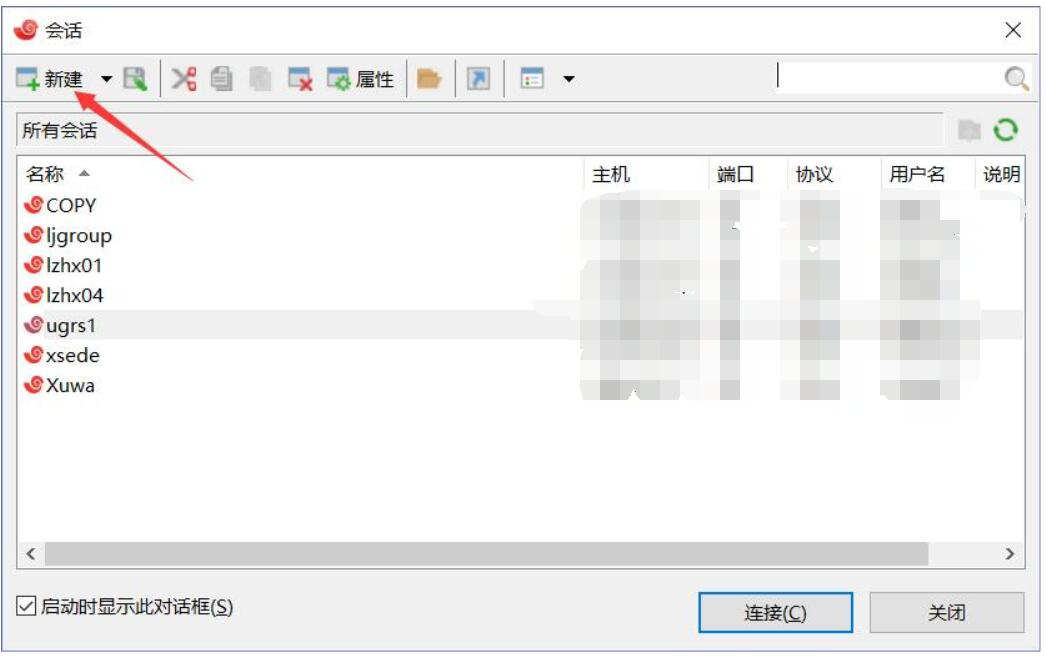
\includegraphics[width = 10cm]{fig/xshell1.jpg}
        \label{XSHELL6打开}
      }
      \subfigure[\textbf{\small{XShell6新建会话窗口}}]
      {
        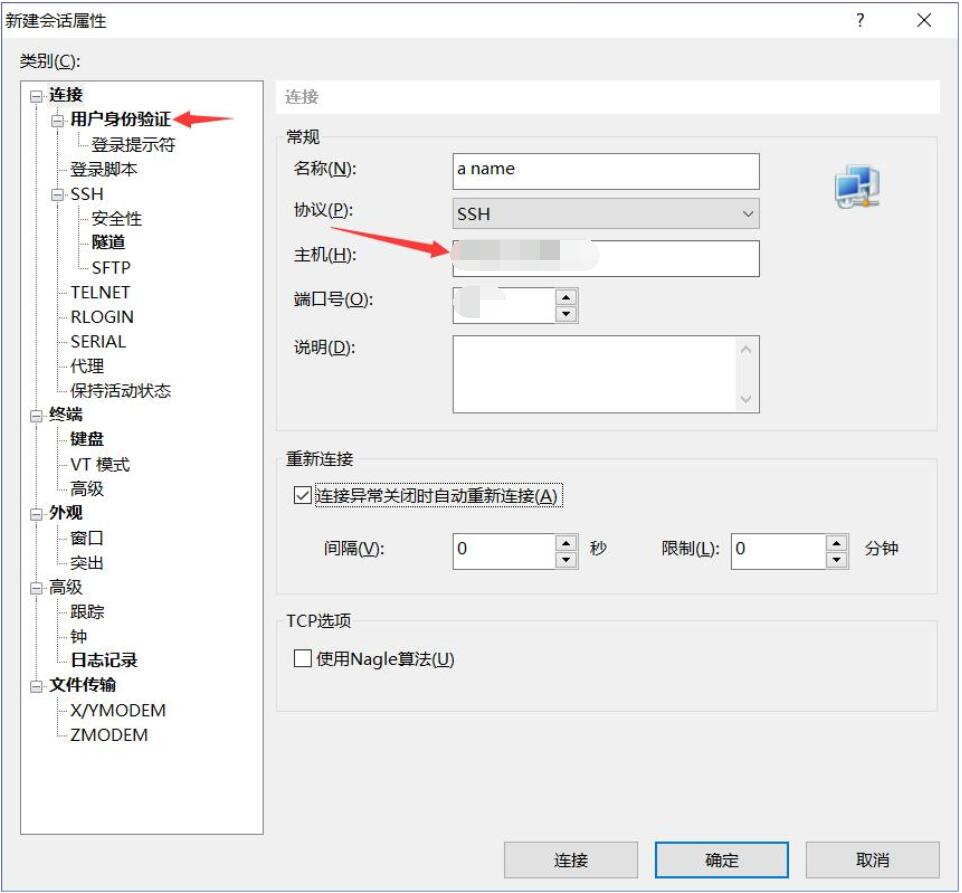
\includegraphics[width = 8cm]{fig/xshell2.jpg}
        \label{XSHELL6新建}
      }
      \caption{\textbf{XShell连接服务器}}
      \label{Xshell}
    \end{figure}
    
    随便起个名字,主机填入10.22.51.200(注意:想要成功连接该IP需要浙大内网:ZJUWLAN、有线网络或者RVPN均可),端口号默认22,在用户身份验证界面用户名输入ugrs3\_LJ,密码为linjungroup\footnote{这个是专为入门本科生注册的账号,主要供学习使用,毕设或者读研读博正式在组内工作会有新的账号}。此时如果见到类似Figure \ref{登录服务器}的界面,就代表已经成功登陆进我们的服务器,并处于\textbf{主目录}(通常用波浪线~表示)下,在光标左侧显示的内容即当前处于ugrs1\_LJ(这个是编者的账号)和tc6000节点(主节点,或称登录节点)。
    \begin{figure}
      \centering
      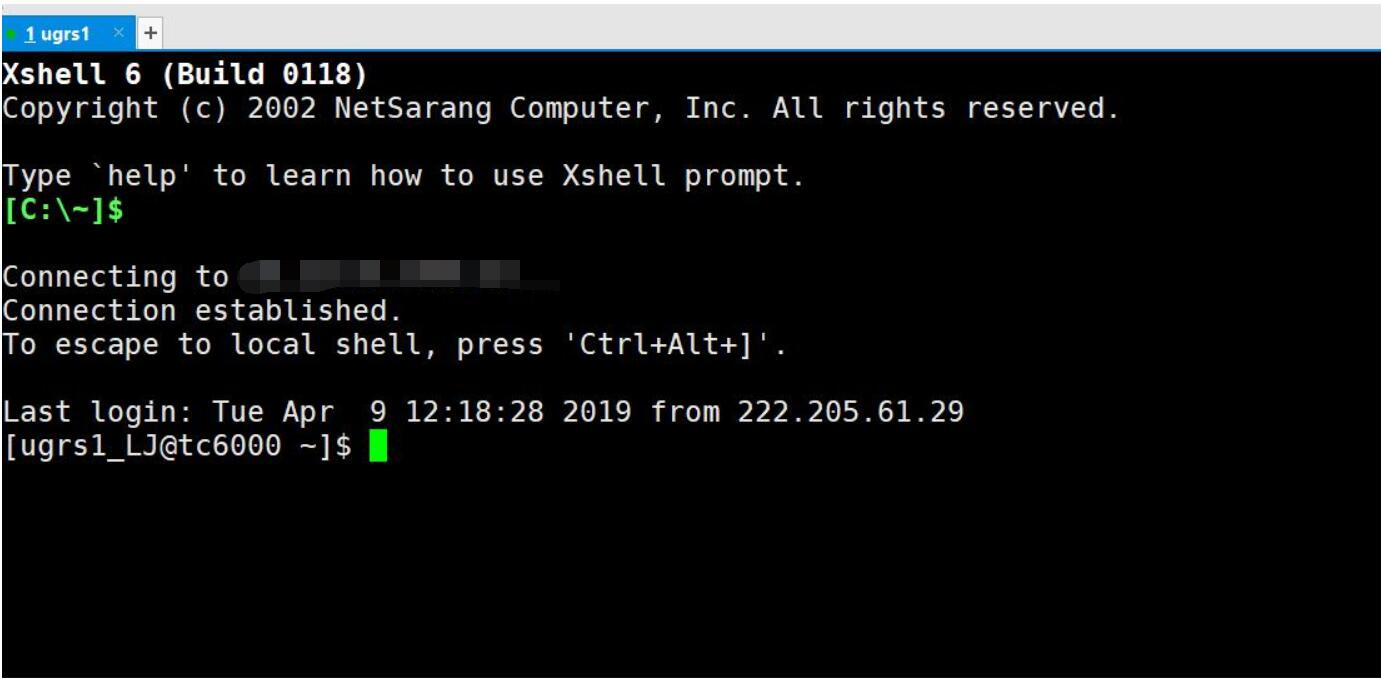
\includegraphics[width = 10cm]{fig/xshell3.jpg}
      \caption{\textbf{成功登陆服务器}}
      \label{登录服务器}
    \end{figure}
    
    登录服务器之后,就可以按照下一小节的内容进行操作,学习Linux系统的各类指令,和如何在Linux系统下编辑文件,为了安全起见,我们建议每个读者在主目录建立自己的文件夹,然后再自己的文件夹中进行各种操作,避免对他人的文件误操作而造成损失。

    \subsection{Linux基本操作}
    \begin{description}
    \item[cd]
      进入输入目录的文件夹;
      `cd folder/'
      P.S : `cd ..' 返回上一级文件夹
    \item[ls]
      列出所在文件夹的子文件夹;

    \item[vi / vim]
      打开文件查看内容;vim事实上是一个文本编辑器(比方说这个文档的一部分也是用vim编辑的)

      P.S :输入不存在的文件可直接创立该文件;

    vim有一个梗,就是几乎所有的人刚上手的时候都不知道\textbf{该怎么退出}。在这里面稍微描述一下最基本的使用方法:
    \begin{description}
      \item[i / Ins] 如果已经打开了某个文本,那么这两个键中的一个能够允许你对文本作出修改。它左下角会显示 ``--INSERT--'' 这样的文段,这说明你处在编辑模式,这时候你按出的大部分操作会如同你使用大部分文本编辑器的时候一样,会完整地呈现在你正在修改的文本上。
      \item[Esc] 无论你处在何种模式,按了Esc你就能回到正常模式,在该模式下你可以用它自身的快捷键来直接作出一些修改,也可输入命令来完成别的操作(比如\textbf{退出})。

      \item[:q!] 这里`:'表示进行对vim程序自身的命令,`q'是quit,`!'表示强制。也就是输了这个命令并按回车后会强制退出并不保存文件。

      \item[:wq] 以此类推,这个表示的是保存并退出。没错,`:w'就是进行保存,并不退出。
    \end{description}
    好了,现在你也是会用vim的人了\footnote{在服务器输vimtutor回车有惊喜!}!跟我一起喊,\sout{vim天下第一!}
    \item[pwd]
      显示所在目录路径;它会显示所处目录的绝对路径,而这个绝对路径是你在任何别的目录下都能访问的。从该角度出发,事实上别的几乎所有操作都可以指定绝对路径(比如简单的访问,或者复制,或者在程序里面调用/生成文件)。

    \item[mkdir]
      在所在目录下建立文件夹:
      `mkdir levest' 表示建立名字为`levest'的文件夹

    \item[cp] 复制文件至某个目录
      `cp einfield.com slot' 表示将`einfield.com' 在`slot'文件夹下进行粘贴

    \item[mv] 原则上它表示将某个东西移动到什么地方,但它的另一个神奇操作在于它可以重命名文件/文件夹(后缀还是要加好)。

    \item[rm] \textbf{ 危险!}这是表示删除操作。

    \item[-r] 在Linux中大部分的`-*' 表示了所进行的主要命令的附加指令(附加属性,\sout{buff})。像这里`-r'一般用来表示是对整个文件夹进行操作,像上面的cp, rm 都可以加上-r。

    \item[*] *一般在Linux表示缺省符号,也就是在这里面可以填任何东西。比方说,`rm *.c' 表示任何后缀为`.c'的文件都会被删除\footnote{这就是为什么sudo rm -rf /* 这个梗会流行的原因。}。

    \end{description}

    读者可以在登录之后所在的主目录下先输入ls和回车,看到当前目录下的文件和文件夹,然后输入“mkdir 文件夹名”的方式创建属于自己的文件夹,然后cd自己的文件夹,之后再这个目录
    下进行后续的操作。
    \subsection{使用服务器递交任务}
    我们的超算集群,简单地说是由很多的CPU(\textbf{节点})构成的,每个CPU有28个\textbf{核},据说服务器的单核运行效率其实是低于正常个人计算机的,但是优势在计算资源非常多。西溪校区的超算集群主要是王林军老师和洪鑫老师出资,也主要是这两个课题组在使用。王老师占有其中的48个节点,共1344个核。这些节点按照一定的顺序组合成了两个\textbf{队列},分别为ljcluster和ljtest,前者又可以分为wenchang和quantum,使用ljclustat指令可以看到全组的节点使用情况。尽管是为本科生学习练习使用的账号,ugrs3\_LJ账号仍然有对服务器三个节点的访问权限(即ljtest队列)。我们在服务器上递交任务,就是将自己的程序交给这些核去运算,要实现这个靠的是PBS任务管理系统。
    
    计算集群是由多台高性能服务器节点组成的,需要有一套系统能够为我们的计算任务自动分配资源,当计算资源出错的时候,能够避免将任务分到异常节点上去,当计算资源全部用完的时候我们再提交任务,能够有一个排队机制当之前的计算任务完成后自动将排处于队状态的作业自动运行。这就是PBS作业调度系统的主要作用。一个常见的PBS任务脚本如下图所示
    \begin{lstlisting}
      #PBS -N 2butene_PBE_0
      #PBS -l nodes=1:ppn=28
      #PBS -q ljcluster
      #PBS -l walltime=99:60:00
      #PBS -j oe
      nprocs=`cat $PBS_NODEFILE | wc -l`
      
      cd $PBS_O_WORKDIR
      cat $PBS_NODEFILE >> NODEFILE
      source /public/software/profile.d/mpi_openmpi-2.0.0-gnu.sh
      source /public/software/compiler/intel2017/mkl/bin/mklvars.sh intel64
      
      python nac.py > nac.out
    \end{lstlisting}

    这是一个调用PBS管理系统的脚本文件,里面的每一行都有其对应的意思,前几行以\#PBS开头的句子为PBS的调度信息相关的指令,-N 代表作业名,这个脚本的作业名为2butene\_PBE\_0,-l 为计算分配资源,图中为分配了一个节点,28个核,注意到第四行也是这类,分配了这个任务的最大运行时间为99小时60分钟(100小时),-q 代表使用哪个队列,图中即为使用ljtest队列,-j 的一行代表将标准输出信息(o)错误信息(e)合并输出到文件。接下来是bash命令行指令,第一行内容为获取本任务所调用的核数,并将这个数赋值给nprocs(在此脚本中此行为多余的,后面并没有用到nprocs),接下来的两行为打开PBS所在目录(也可以使用绝对目录)和将任务占用的节点信息输出到NODEFILE这个文件中,下面两行为环境变量设置,正常情况下不同任务的环境变量设置是不同的,需要根据任务对应的程序而修改,最后一行为执行命令(python)。需要注意,白色的部分为普通的bash脚本,因此可以根据需要任意添加。

    写完PBS文件之后(本例子中文件名即为PBS,可以按需修改),只需要执行“qsub PBS”指令就可以将这个脚本递交给PBS系统,而PBS系统负责根据这个脚本的内容为你分配计算资源,进行计算。希望查看自己的任务,可以使用“qstat”指令,可以打出所有正在服务器运行的任务,希望检索特定队列可以用“-a”,希望进行搜索可以在指令后添加额外的grep指令,举例:如果你希望输出所有在ljtest队列上运行的信息带有ugrs3的任务,指令是“qstat -a ljtest |grep ugrs3”。所有任务的后面会有一个status,R代表正在运行,Q代表正在排队等待运行,C代表运行完成(不代表算对,有可能是由于错误退出),E代表错误退出,H代表被挂起,H的任务即使排队到了资源也不进行计算,先让他之后的任务计算。

    此外,PBS系统还有诸多指令(如常用的qdel和qhold等),诸多功能,诸多环境变量可以调用,鉴于递交任务实际操作的重要性,这里不再赘述,如果在实际操作过程中希望有更多了解,可以参阅浙江大学西溪校区化学系HPC超算平台介绍(可在超算QQ群的群文件中找到)中的Gridview PBS作业调度使用说明。
    
    \section{数学基础}
    \subsection{线性代数回顾及变分法}
    数学基础的第一小节将关注于最基础的数学内容,主要是线性代数的一些知识,由于长时间不用可能有所生疏,我们就在这里作简单的回顾,并且引入变分和线性变分法的概念,熟悉这部分内容的读者可以直接跳过。

    TODO
    \subsection{符号使用}
    在量子力学相关领域,人们使用``左矢''(bra)和``右矢''(ket)来描述一个``状态''。我们可以先简单地认为右矢代表了一个列向量,左矢则代表了一个行向量。它们是这么表示的:
    \[
    | \xi \rangle \rightarrow \text{右矢}, \langle \xi | \rightarrow \text{左矢}    
    .\]  
    我们知道,一个行向量和列向量相乘能够得到一个实数,这也可以理解为两个行向量进行内积的过程,比如两个右矢$| \xi_1 \rangle $ 和$| \xi_2 \rangle $ ,此时它表示为
    \[
    \langle \xi_1 | \xi_2 \rangle 
    .\] 
    当然量子力学远不止于此,它有可能包括了各种奇奇怪怪的东西,使得它并不能完全用向量来描述,比如在线性代数里我们有时候需要用矩阵,在量子力学里它们统统被概括为算符。算符是作用在矢量上的。如果你学过张量分析/矢量代数,你还可以认为它代表了一个张量。有些人们喜欢用$\hat{Q}$类似这样的形式来表达一个算符(也就是加个帽子),也有些人喜欢用粗体,比如$\mathbf{Q}$这样来表达,也有人不加任何东西\footnote{没错就是发明这一套符号系统的\Large{Dirac}大佬。},只要它``在该在的地方''就可以识别为一个算符。算符放在左矢的右边,或者右矢的左边,或者左矢和右矢的中间,也就是
    \[
    \hat{Q}| \xi \rangle ,\langle \xi | \hat{Q}, \langle \xi_1 | \hat{Q} | \xi_2 \rangle   
    .\] 
    到了这里,当然就会出现作用顺序(方向)的问题。不过其实这一套和线性代数非常相像\footnote{事实上这一套就是线性代数——也就是海森堡开发的矩阵力学的核心,量子力学就是线性代数(并不是)},算符默认是作用在右边的,如果需要作用在左矢,那么对应的算符为原算符的厄米共轭(Hermite Conjugate),用$\hat{Q}^\dagger$来表达。那么某种程度上,左矢代表的是右矢的共轭转置,左矢和右矢相作用得到的是两者的内积。

    当然这么说可能很难有感觉这些到底是什么东西,让我们再换一种方式来表达。算符,变换,这些东西实则上都代表了类似于函数的概念,也就是传进去一个东西,传出去另一个东西,这两个东西可以相等,可以完全不是同一类。而左矢和右矢则代表了可以传进去的``参量'',并经过算符作用后得到了另一个左矢或右矢。比如一个关于$x$的函数$f(x)$,经过求导算符$\frac{d }{d x} $作用后得到它的导函数$f'(x)$,实则上也没有脱离这样的描述体系\footnote{从而为Dirac说明海森堡的矩阵力学和薛定谔的波动力学是等价表述做好了铺垫。}。

    \subsection{完备基展开}
    完备基展开是一个非常重要的概念,它直接提供了解决众多微分方程的方法,而解决微分方程是量子力学的至关重要的一个内容。

    ``完备''一词说明某一个基组的完备性,也就是我只要通过这个基组的线性组合就能完整描述我所研究的空间中的所有向量。我用$\hat{x}$,$\hat{y}$,$\hat{z}$三个基向量就能完整描述三维空间里的所有向量,我用${x^n}$便能描述一维的所有函数,我用${\sin{nx},\cos{nx}}$就能描述有限空间内的函数/周期性函数,这些都构成了所谓的完备基。

    在这里请允许编者引入施图姆-刘维尔型方程和对应本征值问题。
    \begin{theorem}
    	对形如
	\begin{equation}
		\frac{d }{d x} \left[ k(x) \frac{d y}{d x}  \right] -q(x)y + \lambda \rho(x) y = 0 \quad (a\leqslant x \leqslant b)
	\end{equation}
	的方程,若$k(x),k'(x),q(x)$ 连续或最多以$x=a$ 和$x=b$ 为一阶极点\footnote{也就是最低项为$\frac{1}{x}$ 项。},则
	\begin{enumerate}
		\item 存在无穷多个本征值
		\[
		\lambda_1 \leqslant \lambda_2 \leqslant \lambda_3 \leqslant ...
		,\] 
		相应地有无限多个本征函数
		\[
			y_1(x),y_2(x),y_3(x),...
		.\] 
		这些本征函数的排列持续正好使节点个数依次增多(即函数值为零的点的个数)。
		\item 所有本征值 $\lambda_n \geqslant 0$,
		\item 相应于不同本征值$\lambda_m$ 和 $\lambda_n$的本征函数$y_m(x)$和$y_n(x)$在区间$[a,b]$上带权重$\rho(x)$正交,即
			\begin{equation}
				\int ^b_a y_m(x) y_n(x) \rho(x) \, dx = 0 
			\end{equation}
		\item 本征函数族$y_1(x),y_2(x),y_3(x)...$是完备的,即函数$f(x)$如具有连续一阶导数和分段连续二阶导数,且满足本征函数族所满足的边界条件,就可以展开为绝对且一致收敛的级数
			\[
				f(x) = \sum_n f_n y_n(x)
			.\] 
	\end{enumerate}
    \end{theorem}
    并由此引入广义傅里叶级数展开
    \[
	    \int ^b_a f(x) y_m(x) \, dx = \sum_n \int f_n y_m(x)y_n(x) \, dx = f_m \int y_m(x)^2 dx   
    .\] 
    即
    \[
	    f_m = \frac{\int ^b_a f(x) y_m(x) \, dx }{\int y_m(x)^2 \, dx }
    .\] 
    这一套系统非常的重要,它能够直接用来解决球坐标下的稳态问题(使用Legendre函数),柱坐标下的稳态问题和动态演化问题(使用贝塞尔函数),以及球坐标下的时间演化问题(使用球贝塞尔函数),其核心内容就在于使用广义傅立叶级数进行展开得到精确解并同时满足边界条件。

    没什么感觉?在这里举一个非常典型的例子,二维传热稳态问题,
    \begin{quote}
	    均匀的薄板占据区域$0<x<a,0<y<\infty$,边界上的温度
	    \[
		    u\big|_{x=0} = 0, u\big|_{x=a} = 0, u\big|_{y=0} = u_0, \lim_{y \to \infty} u =0
	    .\] 
	    求解板的稳定温度分布。
    \end{quote}
    传热这东西,它满足一个扩散方程
    \begin{equation}
	    \frac{\partial u}{\partial t} -a^2 (\frac{\partial ^2 u}{\partial x^2 } + \frac{\partial^2 u}{\partial y^2} + \frac{\partial ^2 u}{\partial z^2}  ) = 0.
    \end{equation}
    稳态,也就是它不随时间变化,$\frac{\partial u}{\partial t} = 0$,而这是二维,所以
    \begin{equation}
	    \frac{\partial ^2 u}{\partial x^2 } + \frac{\partial ^2 u}{\partial y^2 } = 0.
	    \label{2Ddiffusion}
    \end{equation}
    先分离变量,设$u=X(x)Y(y)$,代入(\ref{2Ddiffusion}),左右同除以$u$,
    \begin{equation}
	     \frac{d ^2 X}{X d x^2} = - \frac{d ^2 Y}{Y d y^2} = -k^2 .
    \end{equation}
    由于左边只关于$x$,右边只关于$y$,那么它们只能等于一个常数,考虑到在$x$方向上的边界条件(两边为零,不应该是指数型函数),它们应等于一个负数$-k^2$.
    直接解这个常微分方程,得到
    \begin{equation}
    	\begin{cases}
		X = A_k\sin{kx} + B_k\cos{kx} \\
		Y = C_k e^{-kt}
    	\end{cases}.
    \end{equation}
    由于这个世界实在不太可能有无穷大的温度,故$Y = e^{kt}$项不考虑。

    考虑到$u\big|_{x=0} = u\big|_{x=a} = 0$,$k$应该要满足某种条件才能满足这个,那么事实上
    \begin{equation}
	    X = A_n \sin{\frac{n\pi x}{a}} , k = \frac{n\pi x}{a}, n \in N_+.
    \end{equation}
    由于前面提到的本征值问题,$-k^2$是$X$的常微分方程的本征值,对应本征函数构成完备基,对$Y$也有相应情况,从而$u$可以展开为$XY$的线性组合,即
    \begin{equation}
	    X = \sum_n A_n \sin{\frac{n\pi x}{a}} e^{- \frac{n\pi y}{a}}.
    \end{equation}
    可是……$A_n$怎么确定呀?
    
    就是广义傅立叶级数呀!
    注意到$u\big|_{y=0} = u_0$,有
    \begin{equation}
	    A_n = \int ^a_0 u_0 \sin{\frac{n\pi x}{a}} \, dx = \frac{a u_0}{n\pi} (1-\cos{n\pi}) .
    \end{equation}
    于是我们成功地获得了温度分布的解析解!(?)\footnote{当然有些人会觉得级数展开不算解析解。能展开成简单函数求和已经不容易了。}

    花了这么多篇幅,只是想要说明完备基展开是一个非常重要的内容,它提供了一个解决复杂的微分方程问题的方法\footnote{其实线性代数里的本征值和本征向量也有同样的性质。}。同时它从某种角度上已经道明了量子力学的一个重要的点:
    \begin{center}
    	所有的态都能用本征态的线性组合来表示。
    \end{center}

    哦,我们的读者,然而故事还没有结束呢。

    我们先用曾经描述的量子力学符号来说说这个完备基。对于某个完备的特征值集$\{\lambda_n\}$和特征向量集$\{| e_i \rangle \}$,我们认为特征向量集已经正交归一\footnote{即不同的两个特征向量之间相互正交,且每个向量模为1(即\sout{自交}自己与自己的内积为1)。你可能还记得存在多重特征根的情况,此时你或许也记得这个特征根对应多个特征向量,它们并不一定需要正交。那么你想想就能明白,你能通过某些奇技淫巧让它们互相之间变得正交并仍旧是特征向量(比如大名鼎鼎的Gram-Schmidt 正交化)。},那么有定理
    \begin{theorem}
	\begin{equation}
		\sum \ket{e_i}\bra{e_i} = 1 \, / \, \int dq' \, \ket{q'}\bra{q'} = 1.
	\end{equation}
    \end{theorem}

    $| e_i \rangle \langle e_i | $是一个全新的操作,事实上它其实就是一个算符。为什么呢?因为你可以看到,
    \begin{equation}
	    (| e_i \rangle \langle e_i | ) | \xi \rangle = | e_i \rangle \langle e_i | \xi \rangle = \langle e_i | \xi \rangle | e_i \rangle  .
    \end{equation}
    这是由于$ \langle e_i | \xi \rangle $是一个数,所以它可以游荡在任何地方(向量可以非常自然地乘上任何一个数而不需要管顺序)。也就是我作用于$| \xi \rangle $然后获得了一个新的向量,那么它就是一个算符。

    $1$是沿用了Dirac大佬的写法\footnote{编者表示被Dirac虐得越多\sout{对Dirac越爱得深沉}},就是表示单位算符(或者单位矩阵),作用后得到原来的结果,即
    \begin{equation}
    	1 | \xi \rangle = | \xi \rangle .
    \end{equation}
    所以上面的定理就是在说我把特征向量按照那种方式组合求和后它就会变成单位算符。

    \begin{proof}
    	证明思路:验证其对完备基中任意向量都成立$\Rightarrow$空间内任意向量皆成立

\begin{equation}
	\sum_i \ket{e_i}\bracket{e_i}{e_j} = \sum_i\ket{e_i} \delta_{ij} = \ket{e_j}.
\end{equation}
从而说明该算符对所有特征向量都满足自身为单位算符。

利用展开的唯一性(即一个向量只有一种方式展开/系数组是唯一的),得到
\begin{equation}
\ket{\psi} = \sum c_i \ket{e_i} \Rightarrow c_i = \bracket{e_i}{\psi}.
\end{equation}
因此对所有向量皆满足自身为单位算符。
    \end{proof}
    恭喜你发现了\sout{镇站之宝},展开系数为
    \begin{equation}
    	c_i = \langle e_i | \psi \rangle 
    \end{equation}
    是不是有那么一点感觉?其实就是广义傅立叶级数展开。

    oh忘记说了,$\delta_{ij}$这是(离散)狄拉克函数,它表示$i=j$时其值为1,$i\neq j$时为零。同样地,对于连续狄拉克函数$\delta(x)$,表示$x=0$时其值不为零(或者正无穷),$x\neq 0$时恒为零,同时保证
    \begin{equation}
	    \int \delta(x) \, dx = 1 
    \end{equation}
    它还有这些性质,
    \begin{align}
\delta(-x) & = \delta(x) \\
x\delta(x) & = 0 \\
\delta(a x) & = a^{-1} \delta(x)\\
\delta(x^2-a^2) & = \frac{1}{2} a^{-1} {\delta(x-a)+\delta(x+a)} \quad (a>0)\\
\int \delta(a-x) \, dx \, \delta(x-b) & = \delta(a-b) \\
f(x) \delta(x-a) &=  f(a)\delta(x-a)\\
\int f(x)x\delta(x) \, dx & = 0
\end{align}

    \subsection{傅立叶变换}
  \begin{quote}
    它,改变了世界。
    \begin{flushright}
      ——李睿,谈傅立叶变换时
    \end{flushright}
  \end{quote}     
  还记得傅立叶级数嘛?它长这样:
  \begin{theorem}
  当一个有界函数在$[-l,l]$可积时,该函数可展开为:
  \begin{equation}
    f(x) = \sum_k a_k \cos{\omega_k x} + b_k \sin{\omega_k x}.
  \end{equation}
  其中,
  \begin{equation} 
\begin{cases}
  a_k = \frac{1}{\delta_k l}\int _{-l} ^l f(\xi) \cos{\omega_k} \xi \, d\xi \\
  b_k =  \frac{1}{l} \int _{-l} ^l f(\xi) \sin{\omega_k \xi} \, d\xi 
\end{cases}
.
\end{equation}
其中
\begin{equation}
\omega_k = \frac{k \pi}{l}.
\end{equation}
以及
\begin{equation}
  \delta_k =
  \begin{cases}
  1, \quad k = 0 \\
  2, \quad k \neq 0 
  \end{cases}
  .
\end{equation}
 \end{theorem}

我们刚刚描述过完备基展开,而且$\sin{\frac{k \pi}{l} x}$和$\cos{\frac{k \pi}{l} x}$恰好是 $f''(x) + \lambda f(x) = 0$的解,所以它们在$[-l,l]$上构成了完备基,而且它们互相之间是正交的。在这里值得一提的是,$\sin{\frac{k \pi}{l} x}$满足了\textbf{第一类齐次边界条件},即在边界上函数值为零,而$\cos{\frac{k \pi}{l} x}$满足了\textbf{第二类齐次边界条件},即在边界上的一阶导为零,这允许我们在各类边界条件下研究一个物理问题。同时从某种意义上,我们可以说
\begin{center}
\textbf{边界条件导致了特征值的分立。}
\end{center}
比如在氢原子模型的解里,我们事实上引入了一些“自然边界条件”:在球坐标下的函数必须要满足
\begin{equation}
f(r,\theta, \phi) = f(r,\theta, \phi + 2\pi)
\end{equation}
这引发了角向的特征值分立,也就是\textbf{磁量子数的分立}。

而我们认为波函数在空间的任何一个点都是不发散的,因此在$\theta$方向上必须要展开成多项式而非无穷级数,而$\phi$方向的方程使它必须要符合连属Legendre多项式的形式\footnote{详细讨论还是见任何一本数学物理方法的书。}。同时波函数在全空间下是绝对可积的(因为我们已经定义了波函数的内积——它必须是在Hilbert空间下的),所以在无穷远处它必须收敛于零,这使得径向函数必须满足球Bessel函数的形式。所以从某种角度而言,\textbf{量子力学的能级分立是由于量子力学是使用一个偏微分方程描述且存在边界条件的}。

如果我们想要展开的是一个全实数域的函数呢?令$l \to \infty$,我们发现它转换为一个积分,
\begin{equation}
  f(x) = \int _0 ^\infty A(\omega) \cos{\omega x} \, d\omega + \int _0 ^\infty B(\omega) \sin{\omega x} \, dx  
.
\end{equation}
而系数为
\begin{equation}
\begin{cases}
  A(\omega) = \frac{1}{\pi} \int ^\infty _{-\infty} f(\xi) \cos{\omega \xi} \, d\xi \\
  B(\omega) = \frac{1}{\pi} \int ^\infty _{-\infty} f(\xi) \sin{\omega \xi}\, d\xi 
\end{cases}
.
\end{equation}

我们对它们进行改装,便转化为了复数域中的傅立叶变换以及对应的傅立叶逆变换,即
\begin{equation}
F(k) =  \mathcal{F} [f(x)] = \frac{1}{2\pi}\int_{-\infty}^{\infty} f(x) e^{-ikx} \, dx 
.
\end{equation}
以及
\begin{equation}
  \mathcal{F}^{-1} [F(k)] = \int_{-\infty} ^\infty F(k) e^{ikx} \, dk
\end{equation}
 这便是一般意义下的傅立叶变换\footnote{其实也有不少地方把那个系数$\frac{1}{2\pi}$分摊在正变换与逆变换上。}。我们从完备基上也可以理解,事实上傅立叶变换就是对$e^{-ikx}$进行展开,从而转化为频谱信息。

我们还能够引入各种定理,
\begin{theorem}
\begin{equation}
  \mathcal{F}[f'(x)] = ik F(k)
  \end{equation}
\end{theorem}
\begin{proof}
\begin{align*}
  \mathcal{F}[f'(x)] &=\frac{1}{2\pi}\int ^\infty_\infty f'(x) e^{-ik x} \, dx \\
         &= \frac{1}{2\pi}\left[ f(x) e^{-ik x} \right] ^\infty _{-\infty} - \frac{1}{2\pi}\int ^\infty _{-\infty} f(x) \left[ e^{-ik x} \right] ' \, dx 
\end{align*}
傅立叶变换要求原函数在整个空间上绝对可积,从而有$\lim_{x\to \pm \infty} f(x) = 0$,所以
\[
  \mathcal{F}[f'(x)] = - \frac{1}{2\pi}\int ^\infty_{-\infty} f(x) \left[ e^{-ik x} \right] '  \, dx = ik F(k) 
.\] 
\end{proof}
\begin{theorem}
\begin{equation}
  \mathcal{F}[f(x-x_0)] = e^{-ikx_0} F(k)
\end{equation}
\end{theorem}
\begin{proof}
  \[
    \mathcal{F}[f(x-x_0)] =\frac{1}{2\pi} e^{-ikx_0}\int ^\infty_{-infty} f(x-x_0) e^{-ik(x-x_0)} \, d(x-x_0) = e^{-ikx_0} F(k)
  .\] 
\end{proof}
\begin{theorem}
  \begin{equation}
    \mathcal{F}[f_1(x) * f_2(x)] = 2\pi F_1(k)F_2(k)
  \end{equation}
\end{theorem}
\begin{proof}
  \[
    \mathcal{F}[f_1*f_2] = \frac{1}{2\pi}\int ^\infty_{-\infty} \left[ \int ^\infty_{-\infty} f_1(\xi) f_2(x-\xi) \, d\xi   \right] e^{-ikx} \, dx 
  .\] 
  交换积分次序,
  \[
    \mathcal{F}[f_1*f_2] = \frac{1}{2\pi} \int ^\infty _{-\infty} f_1(\xi) \left( \int ^\infty_{-\infty} f_2(x-\xi) e^{-ik x} \, dx  \right) \, d\xi 
  .\] 
  利用延迟定理,
  \[
    \mathcal{F}[f_1 * f_2] = \frac{1}{2\pi} \int ^\infty_{-\infty} f_1(\xi) e^{-k\xi} \, d\xi \cdot 2\pi F_2(k) = 2\pi F_1(k)F_2(k)
  .\] 
\end{proof}

当然傅立叶变换不只是在一维上。我们对三维空间$\mathbf{r}$也可以做傅立叶变换,
\[
  F(\mathbf{k}) = \frac{1}{(2\pi)^{\frac{3}{2}}} \iiint f(\mathbf{r})  e^{-i\mathbf{k}\cdot\mathbf{r}  } \, d\mathbf{r} 
.\] 

傅立叶变换的一个非常有价值的特点是可以把导数转换为一个常数相乘,从而极大地简化方程。比如无界空间下的扩散问题,
\[
  u_t-a^2u_{xx} = 0
.\] 
初始条件:
\[
  u\big|_{t=0} = \phi(x)
.\] 
傅立叶变换再逆变换就能回到原来的样子,
\[
  u(x,t) = \int \mathcal{F}[u] e^{ikx} \, dk = \mathcal{F}^{-1}[\mathcal{F}[u]]
.\] 
对$x$做Fourier Transform,
\[
  \mathcal{F}[u](k,t) = \frac{1}{2\pi} \int u(x,t) e^{-ikx} \, dx 
.\] 
原方程便转换为
\[
\begin{cases}
  \mathcal{F}[u_t] + a^2 k^2 \mathcal{F}[u] = 0 \\
  \mathcal{F}[u]\big|_{t=0} = \mathcal{F}[\phi]
\end{cases}
.\] 
\[
  \Rightarrow \mathcal{F}[u] = \mathcal{F}[\phi] e^{-k^2 a^2 t}
.\] 
\[
  u = \mathcal{F}^{-1} [\mathcal{F}[\phi] e^{-k^2a^2 t}]
.\] 
有
\[
  \mathcal{F}[f_1 * f_2] = 2\pi \mathcal{F}[f_1] \mathcal{F} [f_2]
.\] 
故
\[
  u = \frac{1}{2\pi} \phi * \mathcal{F}^{-1} e^{-k^2 a^2 t} 
.\] 
当然也可以直接套定义,
\[
  u = \int_{-\infty} ^\infty \mathcal{F}[\phi] e^{-k^2 a^2 t} e^{ikx} \, dk 
.\] 
\begin{align*}
  u &= \frac{1}{2\pi}\int \int \phi(\xi) e^{-ik\xi} \, d\xi e^{ikx}  \, dk\\
    &=\frac{1}{2\pi} \int \phi(\xi) \int e^{-k^2 a^2 t} e^{-ik(x-\xi)} \, dk  \, d\xi \\
    &=\sqrt{\frac{\pi}{a^2 t}}\frac{1}{2\pi} \int \phi(\xi) e^{-\frac{(x-\xi)^2}{4a^2 t}} \, d\xi\\
    &=\frac{1}{2\pi} \phi(x) * \sqrt{\frac{\pi}{a^2 t}} e^{-\frac{x^2}{4 a^2 t}}
\end{align*}
其中,有一步是做配方,
\[
  e^{-k^2a^2 t} e^{ik (x-\xi)} = e^{-a^2 t (k-\frac{i (x-\xi)}{2a^2 t})^2} e^{-\frac{(x-\xi)^2}{4a^2 t}}
.\] 
注意在积分该式时存在积分路径不在实轴的问题,但事实上构造回路后由于回路积分为零,故可以直接化为在实轴上的积分,从而解得最终解。

傅立叶变换实现了函数在实空间和像空间之间的相互转换,而一些算符在两个空间会发生转变(如导数算符转换为常数相乘),使问题能够简化。一个经典的实例就是,
\begin{center}
实空间的波函数在动量空间下的完备基展开就是傅立叶变换。
\end{center}
当然傅立叶变换的意义不止于此,它还代表了信号和频谱之间的转换关系,使其成为信号分析的基础。

薛定谔方程是什么呢?它或许是玄学,它也可能只是一个线性代数的延伸点,它也可能只是一个简单的扩散方程。你可以构建好的完备基来展开对这个体系的描述,你也可以着眼于它的偏微分方程的性质进行求解(比如用格林函数(传播子),比如用傅立叶变换)。这也就是量子力学存在很多学派的原因:量子力学的描述是多种多样的。

王林军老师组存在一个一脉单传(\sout{而且马上就要断了香火})的项目,也就是SMD(旧为PS-QHD —— Phase-Space Quantum Hamiltonian Dynamics)。Moyal得到他的体系便是充分利用了傅立叶变换的这些性质,留给后面叙述。


  \section{量子力学}
  本指南默认入门者对量子力学最基础的部分有一定的理解,因此不会从Schr\"odinger方程入手,也不会涉及五大基本假设。另外,本指南也不涉及高深内容,只有在电子结构部分会从实用的角度简单介绍电子(费米子)的二次量子化。如果你需要量子力学的基础知识,暂时可以参阅各类量子力学教材,但是各类书籍难度差别巨大,我们为初学者推荐Griffiths的量子力学导论,基本看过基础理论部分就已经能满足我们的多数需求。另外,可以参见Levine量子化学中的量子力学基础部分,推导详实。为了方便,我们第一小节为快速概念检索。

  \subsection{快速概念检索}
    \begin{enumerate}
    \item 算符对易子:
    \begin{equation}
    [A,B] = AB - BA
    \end{equation}

    \item 算符对易常用公式:
    \begin{align}
    [A,BC]& = [A,B]C - B[A,C]\\
    [AB,C]& = [A,C]B + A[B,C]
    \end{align}

    \item $x$与$p$的对易关系:
    \begin{equation}
    [x,p]\psi=(xp-px)\psi = -i\hbar[x \frac{\partial}{\partial x}\psi-\frac{\partial}{\partial x}(x\psi)]= i\hbar \psi
    \end{equation}

    \item 波函数是量子态在基组中的投影:
    \begin{equation}
    \psi (x) = \langle x | \psi \rangle , \quad \psi(p) = \langle p | \psi \rangle
    \end{equation} 
  \end{enumerate}
  

  \begin{theorem}
    Ehrenfest Theorem:
    
    \begin{align}
    \mean{\textbf{p}}= m \frac{d \mean{\textbf{x}}}{dt}\\
    \mean{\textbf{F}}= \frac{d\mean{\textbf{p}}}{dt}
    \end{align}
    \end{theorem}

  \begin{proof}
    充分考虑到
    \begin{equation}
    \frac{d\ket{\phi}}{dt}=\frac{1}{i\hbar}[\frac{\textbf{p}^2}{2m}+V(\textbf{x})]\ket{\phi}
    \end{equation}

    \begin{align*}
    \frac{d \mean{\textbf{x}}}{dt}  & = \frac{d \bracketl{\psi}{\textbf{x}}{\psi}}{dt} \\ 
    & = \frac{d\bra{\psi}}{dt} \textbf{x} \ket{\psi} + \bra{\psi} \textbf{x} \frac{d\ket{\psi}}{dt} \\
    &= - \frac{1}{i \hbar}\bra{\psi}[\frac{\textbf{p}^2}{2m}+V(\textbf{x})]\textbf{x}\ket{\psi}+ \bra{\psi}\textbf{x}\frac{1} {i\hbar}[\frac{\textbf{p}^2}{2m}+V(\textbf{x})]\ket{\psi}\\
    &= -\frac{1}{i\hbar}(\frac{\textbf{p}^2}{2m}\textbf{x}-\textbf{x}\frac{\textbf{p}^2}{2m})\ket{\psi}\\
    &= -\frac{1}{2mi\hbar}\bracketl{\psi}{[\textbf{p}^2,\textbf{x}]}{\psi}\\
    &=-\frac{1}{2mi\hbar}\bracketl{\psi}{2\textbf{p}[\textbf{p},\textbf{x}]}{\psi}\\
    &=\frac{1}{m}\bracketl{\phi}{\textbf{p}}{\phi}\\
    &=\mean{\textbf{p}}
    \end{align*}

    \begin{align*}
    \frac{d\mean{\textbf{p}}}{dt} &= \frac{d\bracketl{\psi}{\textbf{p}}{\psi}}{dt}\\
    &=\frac{d\bra{\psi}}{dt} \textbf{p} \ket{\psi} + \bra{\psi} \textbf{p} \frac{d\ket{\psi}}{dt} \\
    &= - \frac{1}{i \hbar}\bra{\psi}[\frac{\textbf{p}^2}{2m}+V(\textbf{x})]\textbf{p}\ket{\psi}+ \bra{\psi}\textbf{p}\frac{1} {i\hbar}[\frac{\textbf{p}^2}{2m}+V(\textbf{x})]\ket{\psi}\\
    &= -\frac{1}{i\hbar}\bracketl{\psi}{[V(\textbf{x}),\textbf{p}]}{\phi} \\
    & = -\frac{1}{i\hbar}\bracketl{\phi}{i\hbar\frac{\partial V(\textbf{x})}{\partial \textbf{x}}}{\phi}\\
    & = \bracketl{\phi}{[-\frac{\partial V(\textbf{x})}{\partial \textbf{x}}]}{\phi}\\
    & = \mean{\textbf{F}}
    \end{align*}

    \begin{align*}
    [V(\textbf{x}),\textbf{p}] \ket{\psi} & = [V(x),-i\hbar \frac{\partial}{\partial \textbf{x}}]\ket{\psi}\\
    & = -i\hbar V(x) \frac{\partial }{\partial \textbf{x}} + i\hbar \frac{\partial}{\partial \textbf{x}}[V(\textbf{x})\ket{\psi}]\\
    &= -i\hbar V(x) \frac{\partial }{\partial \textbf{x}}+ i\hbar \frac{\partial V(\textbf{x})}{\partial \textbf{x}}\ket{\psi} +  i\hbar V(\textbf{x}) \frac{\partial \ket{\psi}}{\partial \textbf{x}}\\
    &= i\hbar \frac{\partial V(\textbf{x})}{\partial \textbf{x}} \ket{\psi}
    \end{align*}
  \end{proof}

  \begin{theorem}
    Hellmann-Feynman Theorem:
    对于依赖某个参数$\lambda$(在本指南的后文中通常为原子核坐标$\mathbf{R}$)的哈密顿算符$\hat{H}_\lambda$本征态$|\psi_\lambda\rangle$,其能量期望值对参数的求导,等于哈密顿量对参数求导再求期望,即
    \begin{equation}
      \frac{\mathrm{d}E_\lambda}{\mathrm{d}\lambda} = \langle\psi_\lambda|\frac{\mathrm{d}\hat{H}_\lambda}{\mathrm{d}\lambda}|\psi_\lambda\rangle
    \end{equation}
  \end{theorem}

  \begin{proof}
    由于$|\psi_\lambda\rangle$是哈密顿算符本征态
    \begin{equation*}
      \hat{H}_\lambda|\psi_\lambda\rangle=E_\lambda|\psi_\lambda\rangle
    \end{equation*}  
    容易得到
    \begin{align*}
      \begin{aligned}
        \frac{\mathrm{d} E_{\lambda}}{\mathrm{d} \lambda}=&\frac{\mathrm{d}}{\mathrm{d} \lambda}\left\langle\psi_{\lambda}\left|\hat{H}_{\lambda}\right| \psi_{\lambda}\right\rangle\\
        =&\frac{\mathrm{d} \langle\psi_\lambda|}{\mathrm{d} \lambda}\hat{H}_\lambda|\psi_\lambda\rangle+\langle\psi_\lambda|\hat{H}_\lambda\frac{\mathrm{d} |\psi_\lambda\rangle}{\mathrm{d} \lambda}+\langle\psi_\lambda|\frac{\mathrm{d}\hat{H}_\lambda}{\mathrm{d}\lambda}|\psi_\lambda\rangle\\
        =&E_\lambda\frac{\mathrm{d} \langle\psi_\lambda|}{\mathrm{d} \lambda}|\psi_\lambda\rangle+E_\lambda\langle\psi_\lambda|\frac{\mathrm{d} |\psi_\lambda\rangle}{\mathrm{d} \lambda}+\langle\psi_\lambda|\frac{\mathrm{d}\hat{H}_\lambda}{\mathrm{d}\lambda}|\psi_\lambda\rangle\\
        =&E_\lambda\frac{\mathrm{d}}{\mathrm{d}\lambda}\left\langle\psi_{\lambda} | \psi_{\lambda}\right\rangle+\langle\psi_\lambda|\frac{\mathrm{d}\hat{H}_\lambda}{\mathrm{d}\lambda}|\psi_\lambda\rangle\\
        =&\langle\psi_\lambda|\frac{\mathrm{d}\hat{H}_\lambda}{\mathrm{d}\lambda}|\psi_\lambda\rangle
      \end{aligned}
    \end{align*}
  \end{proof}

  \begin{description}
	  \item[变分法] 在有限空间中寻找最优解;任意波函数对应的能量期望值都不小于最低本征态能量

	  \begin{theorem}
	    体系的基态能量小于等于体系可能的任意态。
	  \end{theorem}

	  \begin{proof}
	    \begin{align}
	    &\begin{cases}
	    H\ket{\psi_i} = E_i\ket{\psi_i}\\
	    \ket{\psi}=\sum_i c_i \ket{\psi_i}
	    \end{cases}\\
	    \Rightarrow & \bracketl{\psi}{H}{\psi} = \sum_i c_i^* \bracketl{\psi_i}{H \sum_j c_j}{\psi_j} \\
	    =& \sum_{ij}c_i^*c_j E_j \delta_{ij}=\sum_i c_i^* c_i E_i \geq \sum_i c_i^* c_i E_{0}=E_{0}
	    \end{align}
	  \end{proof}

	  \item[微扰法] 尽可能利用简单体系的精确解描述复杂问题
	  \begin{equation}
	    H\ket{\psi_i}=E_i\ket{\psi_i} \quad H=H^{(0)} +\lambda H^{(1)}
	  \end{equation}

	  \begin{align*}
	    &\begin{cases}
	    \ket{\psi_i} = \ket{\psi_i^{(0)}}+\lambda \ket{\psi_i^{(1)}}\\
	    E_i=E_i^{(0)} + \lambda E_i^{(1)}
	    \end{cases}\\
	    \Rightarrow & (H^{(0)}+\lambda H^{(1)})(\ket{\psi^{(0)}_i}+\lambda \ket{\psi_i^{(0)}})=(E_i^{(0)}+\lambda E^{(1)}_i)(\ket   {\psi_i^{(0)}}+\lambda \ket{\psi^{(1)}_i}) \\
	    \Rightarrow & \begin{cases}
	    (H^{(0)}-E_i^{(0)})\ket{\psi_i^{(0)}}=0\\
	    (H^{(0)}-E_i^{(0)})\ket{\psi_i^{(1)}}+(H^{(1)}-E_i^{(1)})\ket{\psi_i^{(0)}} =0
	    \end{cases}\\
	    \Rightarrow & \bracketl{\psi_j^{(0)}}{H^{(0)}-E_i^{(0)}}{\psi_i^{(1)}}=\bracketl{\psi_j^{(0)}}{(E_i^{(1)}-H^{(1)})}{\psi_i^{  (0)}  }\\
	    \Rightarrow & (E_j^{(0)}-E_i^{(0)})\bracket{\psi_j^{(0)}}{\psi_i^{(1)}}=E_i^{(1)}\delta_{ij} -\bracketl{\psi^{(0)}_j}{H^{(1)}}    {\psi_i^{(0)}}\\
	    \Rightarrow &
	    \begin{cases}
	    E_i^{(1)}=\bracketl{\psi_i^{(0)}}{H^{(1)}}{\psi_i^{(0)}} &\quad i=j \\
	    \ket{\psi_i^{(1)}}=\sum_{j\neq i}\frac{\bracketl{\psi^{(0)}_j}{H^{(1)}}{\psi^{(0)}_i}}{E^{(0)}_i-E^{(0)}_j} &\quad i\neq j
	    \end{cases}
	  \end{align*}

	  二阶微扰先略。

	  微扰应用:

	  \begin{equation}
	    T=\frac{p^2}{2m}-\frac{p^4}{8c^2m^3}+....
	  \end{equation}
	  \begin{description}
	  	\item 非谐性:对势能项做微扰
	  	\begin{equation}
	  	V=V(0)+\frac{k}{2}x^2+\frac{\alpha}{6}x^3+\frac{\beta}{24}x^4+...
	  	\end{equation}
	  	\item Stark效应:对外场做微扰
	  	\begin{equation}
	  	H=H_0-\mu\cdot F
	  	\end{equation}
    \end{description}
    
  \end{description}


  \begin{description}
  	\item[全同性原理] 量子世界的全同粒子不可区分,任何两个粒子交换不影响体系的状态;

  	\item[交换算符]
  	\begin{equation}
  	\textbf{P}_{12}[f(q_1,q_2,....,q_n)]=f(p_2,p_1,....,p_n)
  	\end{equation}
  	\begin{equation}
  	P_{12}[1s(1)\alpha(1)3s(2)\beta(2)]=1s(2)\alpha(2)3s(1)\beta(1)
  	\end{equation}

  	\item[交换算符的本征值]
  	\begin{equation}
  	\textbf{P}_{12}[\textbf{P}_{12}[f(q_1,q_2,.....,q_n)]]=f(q_1,q_2,...,q_n)\Rightarrow P_{12}^2=1
  	\end{equation}
  	Thus
  	\begin{equation}
  	c_i=\pm 1
  	\end{equation}

  	交换算符的本征值为实数,只能为$\pm 1$,对应波函数分别称为对称和反对称。不具备对称性的波函数无法用于描述全同粒子。

  	\item[玻色子和费米子] 波函数反对称的粒子为费米子,而波函数对称的粒子为玻色子

  	\item[反对称粒子的泡利不相容原理]
  	\begin{equation}
  	f(q_1,q_1,....,q_n)=-f(q_1,q_1,....,q_n) \Rightarrow f(q_1,q_1,....,q_n)=0
  	\end{equation}
  	\item[自旋统计] Pauli 使用量子场论证明了自旋统计理论,指出费米子(电子和质子等)拥有半整数自旋,而玻色子(光子和声子等)具有整数自旋,电子具有$\frac{1}{2}$的自旋。

  	\item[相对论量子力学] 自旋角动量很自然地以内禀方式蕴含在相对论性狄拉克方程中。作为最低阶非相对论近似,薛定谔方程人为地丢弃了自旋这种相对论效应。量子力学与相对论的完美融合已经超出了量子力学的范围,但是对于单体问题,狄拉克方程严格表述了体系的相对论性质。
  \end{description}
  


\begin{description}
	\item[电流密度]
	\begin{equation}
	j(r)=\frac{1}{2i}\sum_{i=1}^{N}[\grad_i\delta(r-r_i)+\delta(r-r_i)\grad_i]\quad f(r,t)=\bracketl{\psi(t)}{j(r)}{\psi(t)}\end{equation}


	 \item[海森堡方程]
	 \begin{equation}
	 \frac{\partial}{\partial t}j(r,t)=-i\bracketl{\psi(r,t)}{[j(r),H(r,t)]}{\psi(r,t)}
	 \end{equation}


\end{description}

  \section{量子化学-电子结构基础}
    量子化学(电子结构)部分,我们将简要介绍常见的电子结构计算方法,所谓电子结构方法,即求解分子(或者固体)体系的定态Schr\"odinger的方法,大家都知道,多体的SE是难以求得精确的解析结果的,因此量子化学某种程度上也是各类近似方法及其如何一步步逼近精确解的简介,本节会{\color{red}\textbf{简要}}介绍Hartree-Fock理论,DFT理论,post-Hartree-Fock理论(包括组态相关CI,耦合簇方法CC,多组态自洽场方法MCSCF,多体微扰理论等),编者还在最后加入了简化版的电子(费米子)二次量子化的内容。但是限于篇幅,上述理论的证明几乎全部略去。本节内容与王老师高等物理化学-量子化学课程内容相似。
    
    另外,与量子力学章类似,为了方便,我们第一小节作为快速的概念检索使用。

    \subsection{快速概念检索}
    \begin{description}
      \item[BO近似] Born-Oppenheimer近似,电子的运动速度远超过原子核,在解电子的量子力学方程时,核假设不动,反过来,核处于一个电子运动的平均力场下。
       
      \item[自洽场] Self Consistent Field, SCF, 通常是指通过迭代的方法求解波函数的过程,初猜波函数,计算势能,求解新波函数,再计算势能,如此反复直到结果收敛。
      
      \item[平均场近似] 忽略电子动态关联,将电子与电子的相互作用约化成有效的单电子势能,多电子问题转化为单电子问题,多电子波函数简化为单电子波函数的乘积,使用自洽场得到单电子波函数。
       
      \item[Hartree积下的哈密顿量] 
      \begin{align*}
        &\mean{\hat{H}}_{Hartree} \\
        =& \bracketl{\Psi(\{r_i\})}{\hat{H}}{\Psi(\{r_i\})}\\
        =&(\prod_i\bra{\phi_i(r_i)})(\sum_k\hat{h}_k+\frac{1}{2}\sum_{k\neq l}\frac{1}{\hat{r}_kl})(\prod_j\ket{\phi_j(r_j)})\\
        =&\sum_k\bracketl{\phi_k(r_k)}{\hat{h}_k}{\phi_k(r_k)}(\prod_{i\neq k}\bra{\phi_i(r_i)})(\prod_{j \neq k}\ket{\phi_j(r_j)})\\
        &+\frac{1}{2}\sum_{k \neq l}\bracketl{\phi_k(r_k)\phi_l(r_l)}{\frac{1}{\hat{r}_{kl}}\phi_k(r_k)\phi_l(r_l)}(\prod_{i \neq \{k,l\}}\bra{\phi_i(r_i)})(\prod_{i \neq \{k,l\}}\ket{\phi_j(r_j)})\\
        =&\sum_k\bracketl{\phi_k(r_k)}{\hat{h}_k}{\phi_k(r_k)}+\frac{1}{2}\sum_{k \neq l}\bracketl{\phi_k(r_k)\phi_l(r_l)}{\frac{1}{\hat{r}_{kl}}}{\phi_k(r_k)\phi_l(r_l)}
      \end{align*} 

      \item[Slater行列式]
      \begin{equation}
        |\Psi(p_1,p_2,...,p_n)|=\frac{1}{\sqrt{N!}}
        \begin{vmatrix}
        \ket{\phi_1(q_1)} & \ket{\phi_2(q_1)} & ... & \ket{\phi_n(q_1)}\\
        \ket{\phi_2(q_2)} & \ket{\phi_2(q_2)} & ... & \ket{\phi_n(q_2)}\\
        ... & ...& ... & ...\\
        \ket{\phi_1(q_n)} & \ket{\phi_2(q_n)} & ... & \ket{\phi_n(q_n)}\\
        \end{vmatrix}
      \end{equation}
  
      \item[双电子自旋波函数]
      \begin{equation}
        \alpha(1)\alpha(2),\beta(1)\beta(2),\alpha(1)\beta(2),\beta(1)\alpha(2)
        \begin{cases}
        \frac{1}{\sqrt{2}}[\alpha(1)\beta(2)+\beta(1)\alpha(2)]\\
        \frac{1}{\sqrt{2}}[\alpha(1)\beta(2)-\beta(1)\alpha(2)]
        \end{cases}
      \end{equation}
  
    \end{description}
    \begin{description}
    \item[库伦积分]
    \begin{equation}
    \begin{cases}
    \ket{\phi_{1s}^{(1)}}=\frac{1}{\sqrt{\pi}}e^{-r_1}\\
    \ket{\phi_{1s}^{(2)}}\frac{1}{\sqrt{\pi}}e^{-r_2}
    \end{cases}
    \Rightarrow J=(1+\frac{1}{R})e^{-2R}
    \end{equation}
  
    \item[交换积分]
    \begin{equation}
    \begin{cases}
    \ket{\phi_{1s}^{(1)}}=\frac{1}{\sqrt{\pi}}e^{-r_1}\\
    \ket{\phi_{1s}^{(2)}}\frac{1}{\sqrt{\pi}}e^{-r_2}
    \end{cases}
    \Rightarrow K=(\frac{1}{R}-\frac{2R}{3})e^{-R}
    \end{equation}
    它在分子成键中起到了非常关键的作用,是自旋引起的量子效应。

    \item[Koopmans 定理]假设离子轨道与中性分子轨道相同,可计算分子的电离能喝亲和势,改变电子数会引起单电子轨道重排和弛豫,与电子关联量级相似,但符号相反。

    \item[变分法与基组] Hartree-Fock 变分法中,波函数的形式原则上是任意的,但是波函数的随意变化数字处理起来非常麻烦,使用基组对波函数进行线性展开,对量子化学中的所有电子结构计算都至关重要。
  
    \item[原子轨道基组] 完备的基组在量子化学是很难实现的,从计算量的角度需要尽可能地减少基组的数目。氢原子的电子结构可解析求解,为理解更复杂原子和分子的电子结构打开了大门。使用氢原子和类氢离子的原子轨道作为基组,是解决复杂化学问题的通用做法,有着重要的意义。
  
    \item[原子轨道]
    \begin{equation}
      \psi(r,\theta,\phi)=R_{nl}(r)Y_{lm}(\theta,\phi)
    \end{equation}
  
    \item[Slater基组和Gaussian基组]
    \begin{equation}
    \chi(r)\sim e^{-\xi r} \qquad g(r)\sim e^{-\alpha r^2}
    \end{equation}
  
    从物理意义角度看,STO比GTO好;
  
    从波函数积分计算效率角度看,GTO比STO好。
  
    \item[高斯函数线性组合]
    \begin{equation}
    e^{-\xi r}=\frac{\xi}{2\sqrt{\pi}}\int_0^\infty \alpha^{-3/2} e^{-\xi^2/4\alpha}e^{-\alpha r^2} \, d\alpha
    \end{equation}
    \begin{equation}
    \Rightarrow \xi_\mu(r-R_A)\approx \sum_Pc_{p\mu}g_p(\alpha_{p\mu},r-R_p)
    \end{equation}
    \begin{equation}
    \begin{cases}
    g_{1s}(\alpha,r)=(8\alpha^3/\pi^3)^{1/4}e^{-\alpha r^2};\\
    (\alpha,r)=(128\alpha^5/\pi^3)^{1/4}xe^{-\alpha r^2};\\
    g_{3dxy}(\alpha,r)=(2048\alpha^7/\pi^3)^{1/4}xye^{-\alpha^2}
    \end{cases}
    \end{equation}
  \end{description}
  
  \begin{description}
    \item[Dunning 原子轨道基组] 如 aug-cc-pVDZ, aug-cc-pVTZ, aug-cc-pVQZ, aug-cc-pV5Z...
  
    aug:弥散, cc: correlation consistent; p: polarized; V: Valence bonds; DZ: double zeta.
  
    \item[赝势原子轨道基组] 当原子中的电子很多事,内层电子通常对原子性质的影响很小,但是其对应的全电子基组很复杂,为了减少计算量,其贡献可通过有效势能来描述,而且可以包含相对论效应的修正。
  
    \item[赝势基组]
    赝势基组包括赝势和基组两部分,内部电子的贡献采用赝势描述,直接放在哈密顿量里,外层价电子采用一般的基组。
  
    LANL1只考虑加电子,LANL2系列除了加电子外,还考虑次外层电子,因为他们与价层的能查不明显,而且对成键有贡献。
  
    LanL2DZ:对H-Ne使用D95V全电子基组,对Na-Bi使用赝势基组,也就是LANL有效核势加上DZ基组;LanL2DZ是常用基组,适合过渡金属等中等质量的金属元素。
  
    \item[总能量] 变分法保证基组越大,HF能量越小,越接近于精确值。
  
    \item[Hessian矩阵]
    \begin{equation}
    F_{ij}=\frac{1}{\sqrt{m_im_j}}\frac{\partial^2 U}{\partial x_i \partial x_j}
    \end{equation}
  
    \item[振动频率]
    \begin{equation}
    \sum_{j-1}^N (F_{ij}-\delta_{ij}\lambda_k)l_{jk}\Rightarrow det(F_{ij}-\delta_{ij}\lambda_{k})=0
    \end{equation}
  \end{description}
  
  \begin{description}
    \item[电子关联] Hartree-Fock理论中采用平均场处理电子-电子相互作用,缺乏电子之间的关联,电子关联需要用多电子基组展开多体系波函数。
  
    \item[如何有效加入电子关联] 以Hartree-Fock得到的单Slater行列式为基础,考虑多电子关联的主要方法有CI(Configurate Interaction)、MCSCF(Multi-Configured Self-Consistent Field)、MPn、CC(Couple Cluster)等。
  
    HF方法的计算量与电子数的四次方成正比,MP2为五次方,CISD和CCS为六次方,CCSD(T)为七次方,CISDT和CCSDT为八次方,随着电子数增加而迅速增加。
  
    \item[多电子组态] 在Hartree-Fock分子轨道的基础上,所有电子从下到上排列称为Hartree-Fock基态,然后可以将一个电子置于LUMO上得到激发态,基态和各种激发态对应的Slater行列式的波函数统称组态。通常用单激发、双激发、三激发等方式分类。
  
    若有K个分子轨道,每个轨道最多占据两个电子,总电子书数N,则n激发组态数为
    \begin{equation}
    C_N^nC_{2K-N}^n=\frac{N!}{n!(N-n)!}\frac{(2K-N)!}{n!(2K-N-n)!}
    \end{equation}
  
    每个组态都可以用Slater行列式表示。
  
  
    \item[多电子波函数的组态线性组合与CI]
    \begin{align*}
    \ket{\Phi} &= c_0\ket{\psi_0} +\sum_{ra}c_a^r\ket{\psi_a^r}+\sum_{a<b,r<s}c_{ab}^{rs}\ket{\psi_{ab}^{rs}}+\sum_{a<b<c,r<s<t}c^{rst}_{abc}\ket{\psi^{rst}_{abc}}+...\\
    &=c_0\ket{\psi_0} + c_S\ket{S}+c_D\ket{D}+c_T\ket{T}+...
    \end{align*}
  
    Full CI(FCI)包括所有可能的激发,可以给出多电子问题的精确解,
  
    实际上即使我们只考虑有限个单电子基组,所有可能的N-电子基组数目也非常庞大。
  
    通常需要对组态进行阶段,只处理有限个N-电子基组。如只考虑单激发,成为CIS;截断到双激发,成为CISD。
  
  
    \item[组态相互作用关系] 单激发对基态能量没有直接贡献,双激发对基态能量的修正起首要作用,Hartree Fock的本征值问题等价于确保组态与单激发不直接混合,相差两个激发的组态之间没有直接相互作用。
  
    \item[Brillouin 定理]
    \begin{equation}
    \bracketl{\psi_0}{\hat{H}}{\psi_a^r}=\bracketl{a}{\hat{h}}{r}+\sum_b\bra{ab}\ket{rb}=\bracketl{\phi_a}{\hat{f}}{\phi_r}=0
    \end{equation}
  
    \begin{align*}
    \bracketl{\psi_0}{\hat{H}}{\psi_a^r}&=(\prod_i\bra{\phi_i})O_1(\prod_j\ket{\phi_j})\\
    &=\sum_k(\prod_i\bra{\psi{\phi_i}})h_k(\prod_l\ket{\phi_j})\\
    &=\sum_k \bracketl{\phi_k}{h_k}{\phi_k}*\prod_{i \neq k} \bra{\phi_i} \prod_{j \neq k} \bra{\phi_j}\\
    &-\sum_k \bracketl{\phi_k}{h_k}{\phi_k}
    \end{align*}
  \end{description}
  
  \begin{description}
    \item[DFT理论]将电子波函数和体系能量表示为电子密度的泛函,将体系自由度降低,进而进行自洽场计算。
    
    \item[Thomas-Fermi 理论]
      是现代密度泛函理论的雏形,能量期望值完全形成电子密度的泛函,使得电子结构处理变得非常简单。当时其精度有限,因为动能项通过简单的近似得到,而且没有考虑交换和关联对总能量的贡献。
    \item[Hohenberg-Kohn 定理]
    \begin{itemize}
      \item 所有客观测量的期望值原则上都是基态电子密度的泛函。
  
      电子密度分布$\rho(r)$决定了总电子数$N$,从而哈密顿量$H=T_e+U_{ee}+V_{ext}$总只有最后一项可能是不确定的。如果$\rho(r)$是两个不同哈密顿量$H$和$H'$的基态电子密度,而两者的基态波函数分别为$\ket{\Psi}$和$\ket{\Psi'}$,基态能量分别为$E_0$和$E'_0$,基态在不兼并的情况下有
      \begin{equation}
      \begin{cases}
      E_0&=\bracketl{\Psi}{H}{\Psi}\\
      &<\bracketl{\Psi'}{H}{\Psi'}\\
      &=\bracketl{\Psi'}{H'}{\Psi'}+\bracketl{\Psi'}{(H-H')}{\Psi'}\\
      &=E_0'+\int \rho(r)(V_{ext}-V'_{ext})\,dr\\
      E_0'&=\bracketl{\Psi'}{H'}{\Psi'}\\&
      <\bracketl{\Psi}{H'}{\Psi}\\
      &=\bracketl{\Psi}{H}{\Psi}+\bracketl{\Psi}{(H'-H)}{\Psi}\\
      &=E_0-\int \rho(r)(V_{ext}-V'_{ext})\,dr\\
      \end{cases}
      \end{equation}
      Then
      \begin{equation}
      E_0+E'_0<E_0+E_0'
      \end{equation}
      矛盾,故电子密度与唯一的哈密顿量对应。反过来,哈密顿量有唯一的基态电子密度。\footnote{在这里,需要指出的是此定理在基态不兼并的情况下成立。}因此,所有可观测量的期望值都是基态电子密度的泛函,特别地,基态总能量是电子密度的泛函:
      \begin{equation}
      E[\rho]=T_e[\rho]+V_{ext}[\rho]+U_{ee}[\rho]
      \end{equation}
  
      \item 基态电子密度原则上可以通过变分法严格得到。
  
    \end{itemize}
  
    \item[Kohn-Sham密度泛函理论]
    哈密顿量中的动能项难以用密度泛函直接表达,而波函数可以更容易地计算动能,为此1965年Kohn和Sham提出了融合波函数和密度的现代DFT理论,使密度泛函理论成为实际可行的理论方法。
  
    \begin{itemize}
      \item 动能
      \begin{equation}
      T_0[\rho]=\sum_i\bracketl{\phi_i}{-\frac{1}{2}\grad^2}{\phi_i}
      \end{equation}
  
      \item 库伦势
      \begin{equation}
      U_{cl}[\rho]=\frac{1}{2}\iint\frac{\rho(r')\rho(r)}{|r'-r|}\,drdr'
      \end{equation}
    \end{itemize}
  
  \end{description}
  
  
  \begin{theorem}
  The external potential(and hence the total energy) $v(\textbf{r})$, is a unique functional of the electron density $n(\textbf{r})$.
  \end{theorem}
  
  \begin{proof}
  The proof proceeds by \emph{reducio ad absurdum}. 
  
  Assume that another potential $v'(\textbf{r})$, with ground state $\Psi'$ gives rise to the \emph{same} density $n(\textbf{r})$. Now clearly [unless $v'(\textbf{r})-v(\textbf{r})=\mathrm{const}$] $\Psi'$ cannot be equal to $\Psi$ since they satisfy different \sch equations. Hence, if we denote the Hamiltonian and ground-state energies associated with $\Psi$ and $\Psi'$ by $H$, $H'$ and $E$, $E'$, we have by the minimal property of the ground state,
  \begin{equation}
  E'=\bracketl{\Psi'}{H'}{\Psi'}<\bracketl{\Psi}{H'}{\Psi}=\bracketl{\Psi}{H+V'-V}{\Psi}
  \end{equation}
  so that
  \begin{equation}
  E'<E+\int [v'(\textbf{r})-v(\textbf{r})]n(\textbf{r})d\textbf{r}
  \label{ueq1}
  \end{equation}
  Interchanging the primed and unprimed quantities, we find in exactly the same way that
  \begin{equation}
  E<E'+\int [v(\textbf{r})-v'(\textbf{r})]n(\textbf{r})d\textbf{r}
  \label{ueq2}
  \end{equation}
  Addition of \ref{ueq1} and \ref{ueq2} leads to the incosistency
  \begin{equation}
  E+E'<E+E'
  \end{equation}
  Thus $v(\textbf{r})$ is (to within a constant) a unique functional of $n(\textbf{r})$; since, in turn, $v(\textbf{r})$ fixes $H$ we see that the full many-particle ground state is a unique functional of $n(\textbf{r})$.\footnote{PhysRev.136.B864}
  \end{proof}
  
  \begin{theorem}
  The functional that delivers the ground state energy of the system, gives the lowest energy if and only if the input density is the true ground state density.
  
  For any positive integer $N$ and potential $v(\textbf{r})$, a density functional $F[n]$ exists such that
  \begin{equation}
  E_{(v,N)}[n]=F[n]+\iiint v(\textbf{r})n(\textbf{r})\,d^3\textbf{r}
  \end{equation}
  obtains its minimal value at the ground-state density of $N$ electrons in the potential $v(\textbf{r})$. The minimal value of $E_{(v,N)}[n]$ is then the ground state energy of this state.
  
  \end{theorem}
  
  \begin{proof}
  Since $\Psi$ is a functional of $n(\textbf{r})$, so is evidently the kinetic and interaction energy. We therefore difine 
  \begin{equation}
  F[n(\textbf{r})] \equiv \bracketl{\Psi}{T+U}{\Psi}
  \end{equation}
  With its aid we difine, for a given potential $v(\textbf{r})$, the energy functional
  \begin{equation}
  E_v[n]\equiv \int v(\textbf{r})n(\textbf{r})d\textbf{r} + F[n]
  \end{equation}
  It can be easily proved that for a system of N particles, the energy functional of $\Psi'$
  \begin{equation}
  \varepsilon_v[\Psi']\equiv\bracketl{\Psi'}{V}{\Psi'}+\bracketl{\Psi'}{T+U}{\Psi'}
  \end{equation}
  has a minimum at the correct ground state $\Psi$, relative to arbitrary variations of $\Psi'$ in which the number of particles is kept constant. Let $\Psi'$ be the ground state associated with a different external potential $v'(\textbf{r})$. Then,
  \begin{equation}
  \varepsilon_v[\Psi']=\int v(\textbf{r})n'(\textbf{r})d\textbf{r}+F[n']>\varepsilon_v[\Psi]
  \end{equation}
  Thus the minimal property is established relative to all density functions $n'(\textbf{r})$ associated with some other external potential $v'(\textbf{r})$.
  \end{proof}

  \section{非绝热动力学与势间跳跃方法}
    简单的说,量子化学主要分为电子结构理论和动力学,上一大节专注于前者,本节就关注后者,电子结构计算可以给出电子能级的分布,激发态的位置以及其他一系列与之相关的静态性质,而动力学,正如其名,研究电子/原子核在特定情况下随时间的演化,通常化学中的光激发驰豫过程、电荷转移过程、异构化,甚至广义上的所有化学反应都是动力学的范畴。当然很容易想到,动力学的准确性是依赖于电子结构方法的准确性的,随着电子结构理论发展,动力学在研究化学物理等一系列问题中有不可忽视的作用。

    在Born-Oppenheimer近似下,我们可以针对特定的分子构型(核的位置)计算对应的电子能量,对于不同的核坐标$\mathbf{R}$(习惯上大写表示原子核坐标,小写表示电子坐标),可以给出一系列电子能量$U=U(\mathbf{R})$,这就是我们通常所说的势能面。需要注意的是,势能面是基于BO近似的结果,这是一切的前提。
    
    BO近似几乎是量子化学中最重要的近似条件,可以适用于我们平常遇到几乎全部静态问题和很多动态问题,BO近似下基态的势能面也是比较合理的。但是在特定的情况下,尤其是当研究的体系涉及多个激发态——比如光激发然后通过非辐射方式回到基态过程时,BO近似就显示出了其弊端。一类常见的BO近似失效的情况就是圆锥交叉(conical intersections),理想的圆锥交叉指的是两个势能面的至少两个维度在某一分子构型上简并(交叉)。通过早期实验光谱上和理论上的研究,人们发现涉及圆锥交叉的势能面的动力学是BO近似无法描述的。
    
    而此类问题又是化学和物理学中广泛存在的问题,为了解决这类动力学问题,必须把原子核和电子的运动一起加进动力学模拟的过程中,这类动力学通常称为非绝热动力学(non-adiabatic coupling)。处理核的运动有多种方式,经典的分子动力学就是只有原子核的运动,不属于非绝热动力学的范畴,但是经典运动是处理原子核的一种方式,另外还可以将原子核的运动也用量子力学求解,进行全量子的非绝热动力学模拟。王林军老师课题组常用的势间跳跃(surface hopping)方法,就是原子核做经典处理,电子做量子处理的一种混合量子经典的非绝热动力学方法。
      \subsection{非绝热耦合}
        作为“动力学”下的讨论,我们一定会用到含时Schr\"odinger方程:
        \begin{equation}
          i \hbar \frac{\mathrm{d} | \psi \rangle}{\mathrm{d} t}=\hat{H} | \psi \rangle
        \end{equation}
        或者是与之等价的量子Liouville方程:
        \begin{equation}
          \frac{\mathrm{d} \hat{\rho}}{\mathrm{d} t}=\frac{-i}{\hbar}[\hat{H}, \hat{\rho}]
        \end{equation}
        Liouville方程的优点是直接演化密度矩阵(TODO电子结构部分解释),动力学所关心的问题就是波函数/密度矩阵如何随时间演化,而在一般的量子力学语境中,波函数的演化通常是波函数系数的演化,含时的波函数可以写作不含时基组的线性组合
        \begin{equation}
          |\psi(\mathbf{r}, \mathbf{R}, t)\rangle=\sum_{j} c_{j}(t) |\phi_{j}(\mathbf{r} ; \mathbf{R})\rangle
          \label{linear combination}
        \end{equation}
        这个不含时基组可以是(也可以不是)定态Schr\"odinger方程的解,我们讨论一个更一般的情况,这个基组只被要求满足正交归一性,带入含时Schr\"odinger方程得到
        \begin{equation}
          \sum_j c_j \hat{H}|\phi_j\rangle=i \hbar \frac{\mathrm{d} | \psi \rangle}{\mathrm{d} t}=i \hbar\sum_j\left(\dot{c}_j|\phi_j\rangle+c_j\frac{\mathrm{d}}{\mathrm{d}\mathbf{R}}|\phi_j\rangle\dot{\mathbf{R}}\right)
        \end{equation}
        在上式左右两端乘以$\langle\phi_i|$就得到了
        \begin{equation}
          i \hbar \dot{c}_{i}=\sum_{j} c_{j}\left(V_{i j}-i \hbar \dot{\mathbf{R}} \cdot d_{i j}\right)
          \label{time-depend-coeff}
        \end{equation}
        其中定义了$V_{ij}=\langle\phi_i|\hat{H}|\phi_j\rangle$和$d_{ij}=\langle\phi_i|\frac{\mathrm{d}}{\mathrm{d}\mathbf{R}}|\phi_j\rangle$,后者称为非绝热耦合(non-adiabatic coupling,NAC),该项所引发的问题是非绝热动力学的领域核心问题之一。在这里,我们可以通过另一种方式来理解它名字的来源以及它的物理意义:如果我们用最简单的数值方法计算非绝热耦合,即
        \begin{equation}
          d_{ij}=\langle\phi_i|\frac{\mathrm{d}}{\mathrm{d}\mathbf{R}}|\phi_j\rangle\approx\langle\phi_i(\mathbf{R})|\frac{|\phi_j(\mathbf{R}+\Delta\mathbf{R})\rangle-|\phi_j(\mathbf{R})\rangle}{\Delta\mathbf{R}}
          =\frac{\langle\phi_i(\mathbf{R})|\phi_j(\mathbf{R}+\Delta\mathbf{R})\rangle}{\Delta\mathbf{R}}
          \label{numerical dij}
        \end{equation}
        上式的最后结果说明非绝热耦合直接正比于不同核位置的波函数之间重叠,要知道如果这些态在同一个核坐标下满足正交性,当$i\neq j$时不应该有重叠。之所以有不等于0的非绝热耦合,就是因为在不同核坐标下的不同电子态间有“耦合”,而这个耦合正是超越BO近似所引入的,是“非绝热”而引入的。

        非绝热耦合还有另外的性质,它相当于算符$\frac{\mathrm{d}}{\mathrm{d}\mathbf{R}}$,要注意它并非量子力学中的力学量,这是因为它并非一个厄米算符,考虑到动量算符为$i\hbar\frac{\mathrm{d}}{\mathrm{d}\mathbf{R}}$,因此$\frac{\mathrm{d}}{\mathrm{d}\mathbf{R}}$算符是反厄米算符,这等价于对于任意两个态,满足
        \begin{equation}
          d_{ij}=\langle\psi_i|\frac{\mathrm{d}}{\mathrm{d}\mathbf{R}}|\psi_j\rangle=-\langle\psi_j|\frac{\mathrm{d}}{\mathrm{d}\mathbf{R}}|\psi_i\rangle=-d_{ji}
          \label{dij=-dji}
        \end{equation}
        根据上式还可以推出一个平凡的结论$d_{ii}=0$。如果回顾等式(\ref{numerical dij})的结果,可以认为在同一个态的前提下分子约等于$1-1$,最终得到$0$。除去数值方法,还有一种常数的解析求解非绝热耦合的思路。如果$|\psi_i\rangle$和$|\psi_j\rangle$是哈密顿算符的两个本征态,显然有
        \begin{equation}
          \begin{aligned}
            0=\frac{\mathrm{d}}{\mathrm{d}\mathbf{R}}\langle\psi_i|\hat{H}|\psi_j\rangle&=E_j d_{ji}+\langle\psi_i|\frac{\mathrm{d}\hat{H}}{\mathrm{d}\mathbf{R}}|\psi_j\rangle+E_i d_{ij}\\
            d_{ij}&=\frac{\langle\psi_i|\frac{\mathrm{d}\hat{H}}{\mathrm{d}\mathbf{R}}|\psi_j\rangle}{E_j-E_i}
          \end{aligned} 
          \label{analytical dij}
        \end{equation}
        如果知道哈密顿量的形式,对核坐标导数的积分可以直接用来计算非绝热耦合。
      \subsection{绝热表象与透热表象}
        本文中所说的绝热(adiabatic)与透热(diabatic)与热学中相关概念并无直接联系,属于量化领域常用的一种表达。绝热是相对于Born–Oppenheimer近似而言的,需要注意由于翻译的问题,请不要混淆非绝热(non-adiabatic)和透热(diabatic)两个概念。

        根据Troy Van Voorhis在他那篇著名的综述\cite{VanVoorhis2010}中的说法,绝热态定义为BO近似下的哈密顿量的本征态,也就是说在BO近似下解定态Schr\"odinger方程(电子结构计算)得到的波函数就是绝热态,即$\hat{H}|\phi_i\rangle=E_i|\phi_i\rangle$。而透热态是指不随核坐标(分子构型)变化的态,最常用的就是Troy提到的NaCl的例子,透热态其实是量子化学家们为了理解图像和计算的方便提出的不真实存在的量子态,如不管Na和Cl的距离多大,永远为两个中性原子的态,或者是永远是两个离子的态。这样说来十分抽象,但是本质上就是其波函数不随核坐标变化而变化,一个严格的定义为透热态的非绝热耦合为0(甚至很多时候简化为$\frac{\mathrm{d}}{\mathrm{d}\mathbf{R}}|\phi_j\rangle=0$)。在电荷转移中的图像更加清晰,如果电荷转移发生在两个分子间,透热态通常定为电荷局域在第一个分子上的态和局域在第二个分子上的态,而真实的态(电荷分散在两个分子上,也就是绝热态)是两个透热态的线性组合。

        动力学的计算既可以在绝热表象下进行,也可以在透热表象下进行,但是很多时候为了节省计算量,我们不会在每个时刻都计算对应的能量与NAC,而是用某种函数对其进行拟合,每到一个分子构型,只需要用拟合函数计算即可。尽管在实际操作中,绝热态是很容易得到的,因为绝热态是哈密顿量本征态,我们可以用各种电子结构的计算方法得到他们,但是在绝热表象下,两个绝热态之间存在非绝热耦合,势能面间也会有圆锥交叉或者trivial crossing,在交叉点处的非绝热耦合是一个奇点,通常很难用函数拟合或作其他处理,因此人们很多时候会希望通过绝热态的线性组合来构建透热态,在透热表象下进行动力学模拟,这个过程称为透热化(diabatization)。透热化的方法非常多,本向导中也不作仔细的展开,但是根据Troy的综述,真正的透热态是难以通过绝热态线性组合得到的,所以很多文章中会使用构建半透热态(quasi-diabatic state)的说法。需要注意,根据非绝热耦合等于零的定义,透热态按照某个固定的系数的线性组合还是透热态,也就是透热态并不是唯一的,这种不唯一性给了量子化学家构建透热态的更大的自由度。这也是目前透热化的方法多种多样的一个原因。

        在透热表象下,由于透热态不是哈密顿量的本征态,所以此时哈密顿量不再是对角矩阵,而是有非零的非对角元,在某些问题(如电荷转移)中,这些非对角元通常被叫做转移积分(transfer integrals)或者通常称为透热耦合(diabatic couplings, DCs),对角化透热态哈密顿量应该能重新得到绝热态的能量。在透热表象下,可以认为式(\ref{time-depend-coeff})中的$V_{ij}$就是转移积分,所以在某种程度上说,即使透热化并不完全,仍有很小数值的非绝热耦合,只要该项对转移积分是一个小量,对动力学的影响也可以忽略,但是在绝热表象中由于$V_{ij}=0$,因此非绝热耦合即使有些时候较小,仍是十分重要的。
      \subsection{势间跳跃方法与FSSH}
        势间跳跃(Surface Hopping)方法是一种混合量子经典(Mixed-Quantum-Classical)方法\footnote{需要注意混合量子经典与半经典方法(Semi-Classical)不同,
        前者一般指方法中既有经典部分又有量子部分,后者偏向量子力学做经典近似,演化一个半量子半经典的方程},它是非绝热动力学中非常常用的一类,尽管很早就有类似的
        思路,直到1990年John Tully提出了最少跃迁的势间跳跃(Fewest Switches Surface Hopping, FSSH)方法\cite{Tully1990},在这之后surface hopping方法被大量使用并且一直被发展,王老师课题组的核心研究方向就是SH方法中某些复杂问题的处理以及将其往更大体系更多自由度推广。

        在势间跳跃方法,原子核做经典处理,按照分子动力学的方法运动,但是其感受到的势能是由电子势能而非力场提供,电子的势能是根据电子的Schr\"odinger方程描述的,即电子的运动是量子处理。简单地说,如果读者熟悉分子动力学,那么这套方法理解起来是非常容易的,它的思路非常平凡,即在一个某一个时刻开始,在$dt$的时间间隔内用经典方法演化核的运动,然后计算电子波函数在这个$dt$内的演化,电子势能梯度为原子核的运动提供力,进而演化下一个时刻的原子核运动和电子运动,如此重复,就可以得到非绝热动力学的模拟结果。

        当然尽管图像上非常简单,但是实际操作起来会有各种各样的问题,比如下一小节中稍微涉及的势能面交叉和退相干的问题,包括电子如何在势能面上运动,都是现在仍然在讨论的重要问题,我们都会稍作涉及,但是首先要回到最早的FSSH方法上来。

        之所以称为Surface Hopping,就是因为在这套方法中电子的运动其实是在势能面间的跳跃,在特定的时刻内,电子只会存在于其中的某一个势能面(即通常说的active态),不同的SH方法的核心区别通常在于如何定义电子在不同势能面之间的跃迁概率,什么时候会跃迁。当然如果我们研究一个简单的隧穿问题,单一的SH计算只会得到一个固定的结果,要么穿过了势垒要么被反射等等,不会得到具体的隧穿概率数据,因此SH方法通常需要做很多次轨迹,然后取轨迹平均来得到物理观测量的结果。

        在等式(\ref{time-depend-coeff})中,我们演化波函数的系数,但是为了方便,我们会使用密度矩阵的演化,在等式(\ref{linear combination})的展开形式下,密度矩阵的矩阵元定义为$a_{kj}=c_k c_j^*$,在这个两边取时间导数并将(\ref{time-depend-coeff})的结果代入,我们就得到了关键性的等式
        \begin{equation}
          \begin{aligned} i \hbar \dot{a}_{k j}=& \sum_{T}\left\{a_{l j}\left[V_{k l}-i \hbar \dot{\mathbf{R}} \cdot \mathbf{d}_{k l}\right]\right.\\ &-a_{k l}\left[V_{l j}-i \hbar \dot{\mathbf{R}} \cdot \mathbf{d}_{i j}\right] \} \end{aligned}
          \label{time-de DM}
        \end{equation}
        我们通常关心的是密度矩阵的对角元,就是总电子波函数在某个势能面上的\textbf{布居}(\textbf{Population}),令上式中的$k=j$我们得到
        \begin{equation}
          \dot{a}_{k k}=\sum_{l \neq k} b_{k l}
        \end{equation}
        其中
        \begin{equation}
          b_{k l}=2 \hbar^{-1} \operatorname{Im}\left(a_{k l}^{*} V_{k l}\right)-2 \operatorname{Re}\left(a_{k l}^{*} \dot{\mathbf{R}} \cdot \mathbf{d}_{k l}\right)
          \label{time-de DM diagnol}
        \end{equation}
        而$\dot{a}_{k k}$就是势能面$k$上的布居变化,这里我们引入最少跳跃(Fewest Switches, FS)的思想,即在一个时间间隔$\mathrm{d}t$内的布居变化完全由当前态向其他态的跃迁提供,以两个态的体系为例,如果在时间$t$时,假设所有轨迹中电子当前处在1态的轨迹数为$N_1(t)=a_{11}(t)N$,其中$a_{11}$是$t$时刻电子在1态的布居,$N$为总轨迹数。与之类似,我们有$t$时刻处于2态的轨迹数$N_2(t)=a_{22}(t)N$,在很小的时间间隔$\mathrm{d}t$之后,两个布居为$a_{11}(t+\mathrm{d}t)$和$a_{22}(t+\mathrm{d}t)$,不失一般性,我们假设$a_{11}(t)<a_{11}(t+\mathrm{d}t),a_{22}(t)>a_{22}(t+\mathrm{d}t)$,我们就固定这个时间间隔内从态1跃迁到态2的轨迹数为$a_{11}(t+\mathrm{d}t)-a_{11}(t)$,而从态2跃迁到态1的轨迹数为$0$,原则上可以两者各加一个常数,FS的思想等价于固定这个常数为$0$。这样处理之后,我们得到$\dot{a}_{22}=-\dot{a}_{11}=\frac{a_{11}(t)-a_{11}(t+\mathrm{d}t)}{\mathrm{d}t}$,则如下定义的跃迁概率
        \begin{equation}
          P_{1\rightarrow2}\equiv\frac{a_{11}(t)-a_{11}(t+\mathrm{d}t)}{a_{11}(t)}=\frac{\dot{a}_{22} \mathrm{d}t }{ a_{11}(t)}
        \end{equation}
        如果只有两个能级,将等式(\ref{time-de DM diagnol})代入得到
        \begin{equation}
          P_{1\rightarrow2}=\frac{b_{21} \mathrm{d}t }{ a_{11}(t)}
          \label{hopping probability}
        \end{equation}
        上式就是FSSH的核心公式\footnote{细心的读者可能会发现与Tully原文中的分母不完全相同,但是本文的推导更加合理一点,通常也是使用这一套公式,当然,由于$\mathbf{d}t$内密度矩阵几乎不会变化,究竟是用$t$时刻还是$t+\mathbf{d}t$时刻对结果的影响不大。}。FSSH单个轨迹的流程就是先初始化,赋予研究的体系一个初始动能(动量)和位置,然后每个$\mathbf{d}t$内先用经典力学的方法演化原子核的运动,再利用等式(\ref{hopping probability})计算出当前态跃迁到其他态的概率,用随机数的方法判断是否跃迁,同时还要判断跃迁之后是否满足能量守恒,如果满足,则完成跃迁并修正体系原子核运动的速度,不断重复上述过程就得到了动力学演化的结果。
        
      \subsection{鸟瞰SH方法中的特殊问题}
        本小节将会简要地介绍在SH发展这么多年来,出现的很多问题,包括王老师组学长学姐在这方面的工作的简介,但是由于编者水平有限,只能略作介绍,并且有很大概率在细节上理解不全面甚至有错误,而王老师课题组的各位学长学姐在这方面有更多可说的内容。

        \paragraph{Trivial Crossing:}在势能面上演化动力学的过程中,势能面通常会有各类的交叉和相互作用,多数可以归为Trivial Crossing或者Avoided Crossing,两者的定义Figure \ref{two kinds of crossing}所示
        \begin{figure}
          \centering
          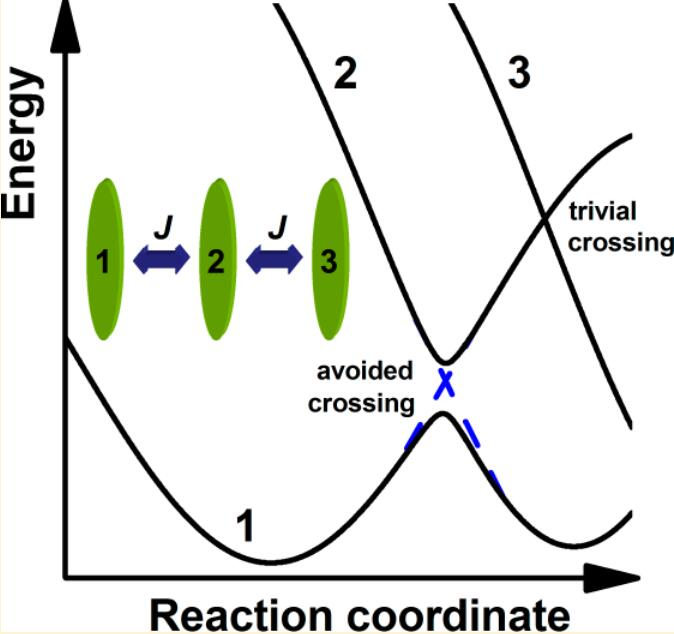
\includegraphics[width = 8cm]{fig/crossing.jpg}
          \caption{\textbf{SH两种Crossing的定义}}
          \label{two kinds of crossing}
        \end{figure}
        图中表示分子1和2之间有相互作用,当它们的势能面交叉时就会产生Avoided Crossing,1和3之间由于距离较远没有相互作用,但是在能量空间下,它们对应的态可能十分接近,这样使得它们的势能面存在交叉,即为Trivial Crossing。另外,Trival Crossing并非只存在于实空间距离很远的两个分子上,即使在同一个分子中,由于轨道之间没有或者相互作用非常小(比如对称性不同的分子轨道,$\sigma$键和$\pi$键之间)但是能量接近,也是可能发生Trivial Crossing的。

        但是由于电子结构计算是按照能量排序的,所以在发生Trivial Crossing的地方会有能级顺序的错误,误将别处毫不相关的能级作为了当前能级,而且根据等式(\ref{analytical dij}),此处的NAC是无法被描述的,通常会由于数值计算时过大而使得跃迁概率接近1,发生不该发生的跃迁,比如从分子1直接跳到分子3。

        为了处理这类问题,王老师发展了很多相关方法,这也是王老师前几年工作的重心。比如SC-FSS和CC-FSSH,后者把常见的Trivial Crossing进行了分类,每一类都有对应的解决方案,基本已经可以处理此类问题,具体内容可以参阅相关文章\cite{wang2014simple}\cite{Qiu2018}\cite{Bai2018}。

        \paragraph{超交换问题:}我们继续用上文中的图,同时联想化学里的过渡态理论,如果只有1态和2态之间、2态和3态之间有相互作用,但是1态和3态之间没有,按照SH方法的处理,如果想从1态到3态必须经过2态,但如果此时2态有较高的能量,高于此时原子核运动的动能,如果跃迁发生,就不满足能量守恒,尽管1态和3态之间的势能差可以被原子核动能满足,由于SH的操作方法,系统是不可能从1态到达3态的。但这并非真实情况,在量子力学中存在隧穿行为,因此实际上体系是会从1态到达3态的,SH这个错误的来源是忽略了原子核的量子效应导致的。当然,这不意味着SH不能处理超交换问题,王老师提出了在Liouville空间下Surface Hopping\cite{wang2015fewest},可以很好地处理超交换和隧穿的问题。

        \paragraph{退相干:}Surface Hopping方法中最大的短板之一就是被称为“过相干(over-coherence)”的现象。为了介绍这种现象,我们先回忆一下FSSH,我们利用运动方程来演化经典的原子核运动和量子的电子演化,这里其实存在一个问题,即使电子的状态和核受力是预先对应好的,但是两者运动的自洽性仍然难以保证。全量子的方法可以保证这个自洽性的存在,SH对原子核的经典处理是过相干现象的缘由。

        在一个单一的轨迹中,不同电子态的电子的运动是一直耦合在一起的,如果在某些情况下,原子核在两个势能面上的受力相差较大,甚至反向,在真实的全量子演化下,两个势能面上的原子核的波包将会分离,这也将导致电子波函数分离成两个部分,不再耦合在一起,然而原始的FSSH方法是无法处理这种退相干(decoherence\footnote{在王老师课题组的文章中有时称为Branching Correction, BC})现象的。因此正确的退相干策略也是SH方法发展的重要主题。
        
        \paragraph{相位修正:}传统的FSSH方法在处理不同势能面的波函数时会有一个相位差的问题。这个问题的来源是当FSSH决定电子要跃迁时,电子是直接跃迁到当前原子核结构下的其他势能面。但是由于势能面的能量不同,其对应的原子核速度不同,以两能级系统举例,如果两个原子核波包同时开始演化,电子一开始位于基态势能面,能量较高的势能面原子核速度较低(这是能量守恒的要求),因此在电子跃迁时,相同相位对应的激发态还未运动到基态波函数对应的位置,而是在其之前,这要求实际操作电子跃迁时,需要对波函数的相位进行修正(Phase Correction)。

    \section{全局优化问题}
      全局优化问题其实是个数学问题,简单地说就是有一个复杂的高维函数,我们如何求得其最小值的问题,但是这个数学问题在化学物理等领域都有重要的意义,我们也主要是全局优化算法在我们的问题中的应用。以最常见的也是王老师课题组之前处理的一个例子,如果任意两个原子之间的相互作用势能是LJ势,给定两个原子,可以通过对坐标求导等于0的方式找到这两个原子的最稳定的位置,但是如果是三个原子,事情就会变得麻烦起来,那如果是一千个原子呢?这个问题其实等价于一个三千维的函数的最小值问题,想通过简单的解析方法求解是几乎不可能的。即使人们有强大的计算机,这样的一个问题还是不简单的,尤其是自由度增多时额外增加的计算量更是不可估计的。人们基于各种各样的思路发展了一系列全局优化算法,限于编者水平,在这里我们只能简单介绍其中的几种。

      我们就以分子原子团簇的优化举例子,我们希望优化的函数是体系总能量。我们先介绍一种最简单的思路,那就是梯度下降,即使是高维函数,你总是可以通过数值的方法求解这一点上能量关于某个自由度的导数(梯度),然后沿着负导数的方向移动,直到达到导数为0为止。这相当于沿着受力的方向一路运动直到达到一个极小值,这种方法的问题也是显然的,就是我们只能达到极小值而非最小值,当自由度非常多时,体系的极小值点可能非常之多,我们一般称这种方法为局部优化,譬如高斯等软件计算分子的最优构型时就是用的类似的思路(当然不是类似LJ势的分子力场的势能,而是量子化学计算的势能)。

      为了尽可能找到极小值,我们需要尽可能搜查整个势能面(直接遍历的计算量是巨大的,但是小体系少自由度情况也可以做),这意味着我们有时需要反着能量下降的方向运动进而跨过一些势垒区域,但是我们又不需要跨越太大的无意义的势垒,解决这个问题就是利用Monte Carlo模拟中接受分子构型的类似方法,认为有一个所谓的温度存在,即不是能量最低原理,而是满足某种分布。在全局优化问题里,我们不一定采用玻尔兹曼分布型的函数,原则上为了达成目的的任何函数形式都可以。当体系沿着某一个自由度能量升高时,用这个函数来判断是否接受构型。

      上面两个思路是全局优化方法的基础,我们通常是多种思路混合得到最后的算法。正如刚刚说的,全局优化算法里可以用遍历的方法寻找最小值,这是最简单粗暴计算量最大的,另一个极端就是完全取随机构型,然后比较取到的随机构型的能量然后从中选中最小的。显然这两种方法都不是特别靠谱,接下来我们介绍一种常用的也是王老师组处理LJ团簇的方法:\textbf{Basin Hopping}。简单的说,这是一种与MC模拟相类似的方法,核心思路为我先有一个初始的分子构型,然后对其进行局部优化得到一个局部优化的结构和对应的能量。然后在这个构型上每个自由度随机移动一点,从这个随机移动得到的构型再做局部优化,如此反复,直接有足够多的极小值,从中挑出最小的那个。这个方法十分简单有效,其随机移动的思路与MC模拟相仿,甚至目的都是一样的:跨过一些势垒尽可能遍历相空间。而王老师课题组还在这里面加入了很多很多为了节省计算量的功能,具体细节只有仔细看过代码才能理解。但是其中非常关键的一部分就是把绝大多数的优化在离散空间内完成,这样原子间的能量就不用每次都计算,而是把离散空间每个格点距离的能量提前算好保存在一个数组里,以后每次使用时只需要调用数组元素就行了。

      另一类比较火爆的思路就是\textbf{遗传算法},这是一个借鉴生物遗传进化的非常有趣的算法。我们首先把分子的结构量化定义为一系列变量,称之为基因,最初,生成一系列随机的结构,称为亲代,然后定义一种“进化”,即用他们的能量函数来表征他们的生存优势,经过一次次筛选,只有能量更低的(生存优势更大)的分子会留下。然后这些有优势的分子进行“杂交”,将他们的结构按某种方法进行组合生成新的子代分子,子代的分子之间再按照某种方式进行筛选,留下能量更低的分子,再进行“杂交”,如此反复,最后就能得到能量较低的“进化”之后的分子。

      向生物学习也是全局优化中的常见思路,除了遗传算法之外,现在还有基于蚂蚁寻找食物思路的算法等,不予详细介绍。另外,可以看出,机器学习在这方面也肯定有一定的建树,但是势能面通常过于复杂,简单的机器学习网络可能无法实现。

      当然,全局优化的问题远远不限于分子能量优化上,包括求条件极值,减小误差,拟合等多种问题都可以使用全局优化的思路进行处理,有时候往往能产生有趣的效果。\sout{初一看只有一两个做全局优化的学长学姐,做到最后就会发现,组内一大半的人都在做全局优化}

      \bibliographystyle{unsrt}
      \bibliography{reference}
  \end{document} 

